\chapter{Resultados Parciais}\label{sec:resultados}
Neste capítulo os resultados parciais são apresentados divididos nas seguintes seções. A Seção \ref{sec:prova} destaca pontos relevantes de um artigo publicado no Simpósio Brasileiro de Informática na Educação (SBIE) responsável em nortear esta proposta entitulado como Framework para coleta e inferência de estados emocionais de estudantes. A Seção \ref{sec:avalexp} apresenta um estudo experimental sobre as arquiteturas de redes neurais de convolução envolvendo o domínio do problema e enquanto a Seção \ref{sec:considera} o resumo deste capítulo.   


%\section{\textit{Framework} para coleta e inferência de estados emocionais de estudantes}\label{sec:prova}
\section{Prova de Conceito}\label{sec:prova}
Inicialmente, uma prova de conceito foi realizada para nortear o andamento deste projeto. Este trabalho \citep{cruz2017framework} consistiu na utilização da API da \textit{Microsoft Cognitives Services}, um serviço na nuvem que oferece um conjunto de aplicações cognitivas, inclusive um reconhecedor de emoções via expressão facial. Esta experiência foi bastante positiva possibilitando ponderar as vantagens e desvantagens desta API, e assim, nortear a construção do reconhecedor de emoções proposto. A contribuição principal deste trabalho está em reconhecer emoções em tempo real, em um cenário real e de forma automática, correlacionando as emoções detectadas com o desempenho escolar em um teste. 

A revisão sistemática (ver Capítulo \ref{sec:revisaosistematica}) mostrou que os pesquisadores da área de reconhecimento de emoção ainda estão tímidos para colocar esses reconhecedores no mundo real. Desta forma, a utilização em cenários reais passa a ser um ponto de contribuição, atestando que essas tecnologias estão amadurecidas possibilitando a integração com outros sistemas, principalmente para tomadas de decisão, recomendações, análises de comportamento e entre outros. Contudo, alcançar precisão no cenário real não é uma tarefa trivial, visto que o reconhecedor deve alcançar uma excelente taxa de generalização. O mundo real é desafiador por haver muitas variações da face e do ambiente dificultando a precisão do algoritmo.  

\subsection{Síntese}
Neste artigo \citep{cruz2017framework}, propomos um \textit{framework} para detectar estados emocionais de alunos baseado em reconhecimento de expressões faciais no contexto das plataformas digitais educacionais. Analisamos e discutimos o uso de correlação e entropia entre os estados emocionais dos estudantes e o desempenho durante uma avaliação de múltipla escolha. Realizamos um experimento com 27 estudantes e elaboramos um teste composto de 40 perguntas. Na análise dos dados correlacionamos os estados emocionais de neutralidade, tristeza, felicidade, raiva, desgosto, medo, desprezo e surpresa, detectados com o desempenho no teste. Concluímos que as questões que ocorreram maior variabilidade das emoções tinham também as maiores proporções de acertos.

\subsection{Objetivos}
O artigo \citep{cruz2017framework} tem como objetivo: (i) propor uma arquitetura de detecção automática de emoções para ambientes educacionais digitais por meio de reconhecimento automático de expressões faciais, utilizando processamento de imagens, de modo a tornar possível a obtenção de dados emocionais dos alunos durante o processo de aprendizagem, e (ii) analisar por meio de estatística descritiva um estudo de caso com dados obtidos a partir desta arquitetura. Esta análise pretende investigar e medir correlações entre as emoções e o desempenho obtido nas questões, levantando hipóteses relevantes sobre a relação entre os estados emocionais e o desempenho, o qual é relevante para sistemas de recomendações, tutores inteligentes e heurísticas em geral, que se interagem de forma dinâmica com as necessidades de aprendizado de cada aluno.

\subsection{Metodologia Experimental}
Um experimento foi realizado com 27 alunos do Ensino Médio de uma escola de tempo integral que farão o Exame Nacional do Ensino Médio (ENEM) 2017. O experimento consistiu em um simulado do exame contendo 40 questões de múltipla escolha.

\subsubsection{Planejamento}\label{sec:plan}
Adotamos uma plataforma educacional que permite a execução de questionários de múltipla escolha, coleta de cliques efetuados pelo estudante, captura automática de foto via câmera frontal do dispositivo, seja por \textit{tablet}, \textit{smartphone} ou \textit{notebook}. Os assuntos escolhidos foram: matemática, língua portuguesa, química, raciocínio lógico, geografia e história. O simulado teve duração de duas horas e cada questão possuía dois níveis de dificuldade (fácil ou difícil), além de ter cinco respostas alternativas.

Para o componente classificador, selecionamos a API da \textit{Microsoft Cognitives Services}, justamente por classificar bem emoções como neutralidade, felicidade e tristeza. Acreditamos que, no contexto da educação, uma emoção bastante comum é a neutralidade, pelo fato da expressão facial do estado de concentração se assemelhar bastante com a expressão facial de neutralidade reconhecida por esta API. Constatamos que estudantes quando estão pensando, estão concentrados, emitindo poucas movimentações intensas e variações de suas expressões faciais, assemelhando-se com a expressão de neutralidade.

\subsubsection{Execução}
A seleção dos estudantes para participar do experimento ocorreu voluntariamente. O grupo final formado foi heterogêneo, onde 53\% consideravam até o momento seu desempenho na escola como bom ou ótimo e, 47\% como regular ou ruim; além disso, 30\% deles consideravam a sua preparação para o vestibular como boa ou ótima e, 70\% como regular ou fraca. Os alunos selecionados são de turmas diferentes.

\subsection{Resultados e Discussões}
Inicialmente, obtemos os seguintes atributos calculados como os valores médios por questão, utilizando os dados coletados dos vinte e sete alunos: (i) a proporção de acertos; (ii) o nível de dificuldade; (iii) a média das probabilidades para cada emoção detectada; e (iv) a entropia por questão. Assim, obtemos um total de onze atributos (resumidos na Tabela \ref{tabelaArti}), onde cada um deles é representado por uma variável aleatória com quarenta valores.

Posteriormente, aplicamos a correlação de Pearson para analisar se há qualquer grau de correlação entre os pares dos atributos mencionados. A Tabela \ref{tabelaArti} apresenta a correlação entre a média das probabilidades de cada emoção com o nível de dificuldade e a proporção de acertos. Os principais resultados estão destacados em negrito.

Como podemos verificar na Tabela \ref{tabelaArti}, a expressão facial neutra possui uma correlação negativa com a proporção de acertos dos alunos (segunda coluna da Tabela \ref{tabelaArti}). Isto indica que estimular emoções diferentes da neutralidade durante a avaliação favorece o desempenho dos alunos. Um segundo indicativo de que isto ocorre, é dado pela correlação positiva entre o desprezo e a felicidade com a proporção de acertos e, de forma discreta, também ocorre com tristeza, surpresa e medo.

A entropia é calculada a partir do valor das probabilidades das emoções detectadas. Logo, percebemos que quando a neutralidade baixa, a entropia aumenta, o que significa que outras emoções estão sendo detectadas com maior probabilidade, ocorrendo a dispersão dos estados emocionais. Portanto, o fato de existir uma correlação positiva entre o aumento da entropia e a proporção de acertos reforça a observação constatada no parágrafo anterior. Adicionalmente, descobrimos que a emoção mais frequente foi a neutralidade, devido aos alunos passarem a maior parte do tempo concentrados analisando as questões para a busca de soluções. Assim, quando o nível de dificuldade da questão aumenta, a neutralidade também aumenta, isto pode ser um indício de que questões mais difíceis tem tendências de exigir maiores níveis de concentração do estudante.

Podemos considerar a hipótese de que, quando o estudante está respondendo uma questão, ao selecionar uma resposta, o mesmo tem uma percepção se acertou ou errou e, nesse momento, há possibilidade de emitir emoções positivas como felicidade e surpresa, ou emoções negativas como tristeza ou desprezo. Portanto, há uma variação dos estados emocionais durante o tempo de resposta de cada questão que deve ser considerado como um problema de mudança de estados. Este resultado é reforçado por
questões que ocasionaram maior entropia, ou seja, quanto maior a dispersão das emoções, maior é o índice de proporções de acertos.

A emoção desprezo aumenta a medida que as questões têm maiores proporções de acertos, isto pode ser explicado, pela mudança de estados durante o tempo de resposta de cada questão ou pelo fato da expressão facial de desprezo se assemelhar com a expressão facial de felicidade. Neste caso, é bem provável estar ocorrendo confusão por parte do classificador em diferenciar felicidade e desprezo.

\begin{table}[]\footnotesize
\centering
\caption{Resultado​ ​da​ ​correla\c{c}\~ao​ ​de​ ​Pearson​ ​para​ ​cada​ ​emo\c{c}\~ao​ ​detectada
e​ ​a​ ​entropia​ ​contra​ ​os​ ​atributos​ ​das​ ​quest\~oes}
\label{tabelaArti}
\begin{tabular}{|c|c|c|}
\hline
                      & \textbf{Nível de Dificuldade} & \textbf{Proporção de Acertos} \\ \hline
\textbf{Tristeza}     & \textbf{-0.33}                & 0.27                          \\ \hline
\textbf{Neutralidade} & \textbf{0.36}                 & \textbf{-0.48}                \\ \hline
\textbf{Desprezo}     & -0.15                         & \textbf{0.30}                 \\ \hline
Desgosto              & -0.13                         & 0.07                          \\ \hline
Raiva                 & -0.14                         & -0.08                         \\ \hline
Surpresa              & 0.07                          & 0.24                          \\ \hline
Medo                  & -0.06                         & 0.14                          \\ \hline
\textbf{Felicidade}   & -0.14                         & \textbf{0.31}                 \\ \hline
\textbf{Entropia}     & -0.12                         & \textbf{0.36}                 \\ \hline
\end{tabular}
\end{table}


Tanto a arquitetura para o reconhecimento de estados emocionais, como a
realização de análises de estados emocionais de estudantes, são úteis para a implementação de tutores inteligentes e sistemas de recomendações que possam fornecer personalização mais precisa do conteúdo para cada aluno levando em consideração seus estados emocionais. É importante identificar os casos diferentes da expressão neutra, justamente por serem menos frequentes podendo indicar alguma oportunidade de um tutor inteligente atuar.

%Como trabalho futuro, pretendemos investigar a mudança temporal dos estados emocionais do estudante, mediante a estímulos produzidos por diferentes objetos de aprendizagem durante uma aula. Também, a implementação de uma heurística que considera o estado emocional do estudante para fornecer ajuda sob demanda com a intenção de aumentar o engajamento e o desempenho durante uma aula.

Finalmente, percebe-se que o \textit{framework} para classificação automática de emoções a partir de imagens necessita de um maior volume de dados, para reduzir eventuais erros de classificação, e permitir a classificação de novos tipos de emoções. Portanto, está nos nossos planos investigar alternativas para amenizar erros de classificação e melhorar a acurácia do \textit{framework}.



\begin{comment}
\section{\textit{Framework} para coleta e inferência de estados emocionais de estudantes}\label{sec:prova}
Inicialmente, uma prova de conceito foi realizada para nortear o andamento deste projeto. O resultado desta prova de conceito foi publicada no Simpósio Brasileiro de Informática na Educação (SBIE) 2017 \citep{cruz2017framework}. Este trabalho consistiu na utilização da API da \textit{Microsoft Cognitives Services} um serviço na nuvem que oferece um conjunto de aplicações cognitivas, inclusive um reconhecedor de emoções via expressão facial. Esta experiência foi bastante positiva possibilitando ponderar as vantagens e desvantagens desta API, e assim, nortear a construção do reconhecedor de emoções proposto. A contribuição principal deste trabalho está em reconhecer emoções em tempo real, em um cenário real e de forma automática, com precisão aceitável em um ambiente educacional, correlacionando as emoções detectadas com o desempenho escolar em um teste. 

A revisão sistemática (ver Capítulo \ref{sec:revisaosistematica}) mostrou que os pesquisadores da área de reconhecimento de emoção ainda estão tímidos para colocar esses reconhecedores no mundo real. Desta forma, a utilização em cenários reais passa a ser um ponto de contribuição atestando que essas tecnologias estão amadurecendo possibilitando a integração a outros tipos de sistemas principalmente para tomadas de decisão, recomendações, análises de comportamento e entre outros. Contudo, funcionar no cenário real não é uma tarefa trivial, o reconhecedor deve alcançar uma excelente taxa de generalização, o mundo real é desafiador por haver muitas variações da face e do ambiente dificultando a precisão do algoritmo.  

\subsection{Síntese}
Neste artigo \citep{cruz2017framework}, propomos um \textit{framework} para detectar estados emocionais de alunos baseado em reconhecimento de expressões faciais no contexto das plataformas digitais educacionais. Analisamos e discutimos o uso de correlação e entropia entre os estados emocionais dos estudantes e o desempenho durante uma avaliação de múltipla escolha. Realizamos um experimento com 27 estudantes e elaboramos um teste composto de 40 perguntas. Na análise dos dados correlacionamos os estados emocionais de neutralidade, tristeza, felicidade, raiva, desgosto, medo, desprezo e surpresa detectados com o desempenho no teste. Concluímos que as questões que ocorreram maior variabilidade das emoções tinham também as maiores proporções de acertos.

\subsection{Objetivos}
O artigo \citep{cruz2017framework} tem como objetivo: (i) propor uma arquitetura de detecção automática de emoções para ambientes educacionais digitais por meio de reconhecimento automático de expressões faciais, utilizando processamento de imagens, de modo a tornar possível a obtenção de dados emocionais dos alunos durante o processo de aprendizagem, e (ii) analisar por meio de estatística descritiva um estudo de caso com dados obtidos a partir desta arquitetura. Esta análise pretende investigar e medir correlações entre as emoções e o desempenho obtido nas questões, levantando hipóteses relevantes sobre a relação entre os estados emocionais e o desempenho, o qual é relevante para sistemas de recomendações, tutores inteligentes e heurísticas em geral, que se interagem de forma dinâmica com as necessidades de aprendizado de cada aluno.

\subsection{Método Proposto}
A arquitetura proposta na Figura \ref{fig:metproposto} é formada pelos seguintes componentes: (i) uma plataforma educacional digital executada, por exemplo, em um \textit{tablet} com câmera frontal que possibilite a coleta de imagens das expressões faciais e das atividades dos alunos, relacionadas com a seleção das respostas e a navegação entre os diferentes objetos de aprendizagem; (ii) um classificador de emoções que recebe como entrada as imagens das expressões faciais e retorna um vetor com as probabilidades a posteriori das seguintes emoções: neutralidade, surpresa, felicidade, tristeza, desprezo, raiva, medo e desgosto; e (iii) um conjunto de métodos de estatística descritiva para realizar diversas análises úteis para: inferências, heurísticas, sistemas de recomendações, tutores inteligentes e inclusive para auxiliar o professor na tomada de decisões referentes às dificuldades de aprendizagem de cada aluno. A arquitetura proposta pode ser usada em tempo real, tanto em ambientes presenciais como à distância, possibilitando o cruzamento dos estados emocionais com a interação na plataforma.

\begin{figure}
\centering
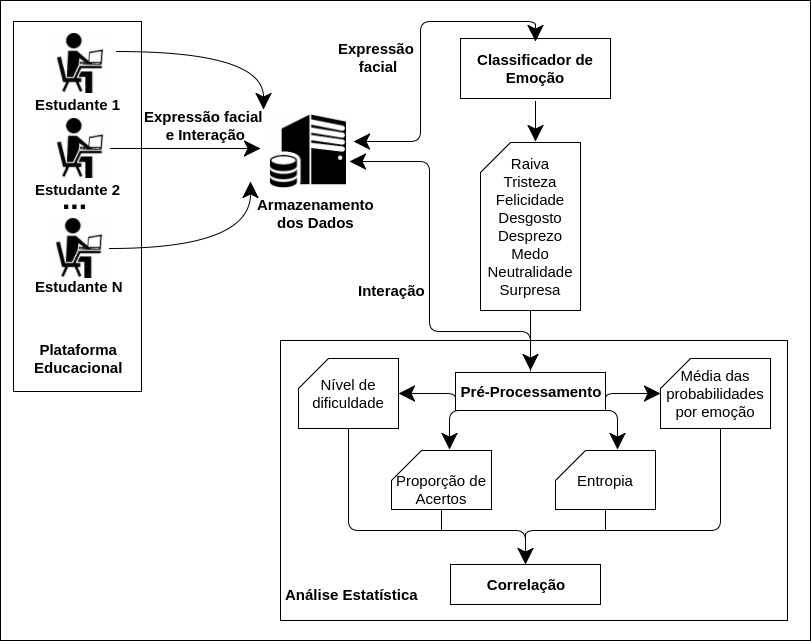
\includegraphics[scale=0.5]{figuras/diagrama.png}
\caption{Método Proposto}
\label{fig:metproposto}
\end{figure}

\subsubsection{Plataforma Educacional}
A plataforma educacional deve possuir um módulo coletor de dados que armazene continuamente os eventos da interação do estudante, tais como, a seleção das questões e suas respectivas respostas, e a identificação de todos os itens presentes na interface como botões, caixa de texto, opções de seleções e outros, assim como, a captura contínua da expressão facial do estudante.

Estes dados são armazenados para tornar possível diferentes análises, tais como: qual foi a emoção predominante na questão que os alunos mais erraram? Na questão que houve mais trocas de respostas qual foi a emoção predominante? Qual foi a emoção predominante no grupo de alunos que mais erraram as questões? Quais as emoções têm ocorrências na variação da dificuldade das questões? Isto pode ser um caminho para inferir a confusão via expressão facial que é um estado emocional não pertencente ao grupo das emoções básicas, entretanto, muito comum em ambiente educacional verificado por \cite{d2013beyond} que em alguns estudos de casos, concluíram que a confusão, tédio, curiosidade, engajamento, frustração e satisfação ocorrem cinco vezes mais do que as emoções básicas no âmbito educacional.

\subsubsection{Classificador de Emoção}
O classificador de emoção tem a função de identificar nas imagens as expressões faciais e atribuir um rótulo a cada imagem. Estes rótulos podem ser: neutralidade, raiva, felicidade, tristeza, desgosto, desprezo, medo e surpresa, como mencionado por \cite{ekman1994}, que são as emoções básicas capazes de ser reconhecidas dada uma expressão facial.

O classificador utilizado está descrito na Seção \ref{sec:plan}, e usufrui de técnicas de aprendizagem de máquina, mais especificamente de aprendizagem profunda em redes neurais pela arquitetura \textit{Convolutional Neural Network} (CNN), que tem sido o estado da
arte para este fim.

A saída do classificador de emoção para cada imagem recebida é um vetor de probabilidades que contém a probabilidade de cada emoção detectada na imagem \textit{i.e.: P=\{p\textsubscript{1},p\textsubscript{2},..,p\textsubscript{n}\}}, onde \textit{p\textsubscript{n}} representa a probabilidade a posteriori da detecção da n-ésima emoção. Uma propriedade é que a soma das probabilidades é igual a 1, e que a maior probabilidade presente no vetor corresponde ao rótulo final da emoção detectada na imagem, ou seja, a sua classificação \textit{e.g.: emoção = max(P)}.

\subsubsection{Análise Estatística}
Este componente contém outros subcomponentes que realizam análises acerca do desempenho e das emoções do estudante por meio da correlação de Pearson. Todos os subcomponentes recebem como entrada tanto os cliques de interação do estudante com a plataforma, como as classificações das expressões faciais. Desta forma, são recuperadas todas as instâncias necessárias para a realização do cruzamento da interação da plataforma com a emoção detectada, a fim de obter o coeficiente de correlação.

Um pré-processamento dos dados é executado antes da análise, onde é organizada a coleção de dados por questão, isto é, a reunião de todas as instâncias de todos os alunos com respeito a uma determinada questão e, desta forma, são agrupados a interação com a plataforma e os dados das classificações de emoções por questão. O
pré-processamento produz as seguintes informações para cada questão:

\begin{itemize}
 \item a média das probabilidades para cada emoção, incluindo todos os alunos;
 \item o nível de dificuldade;
 \item a proporção de acertos, por exemplo, se a metade dos alunos acertaram, então a
proporção é 50\%; e
 \item a entropia das emoções, que mede a dispersão das probabilidades das emoções
detectadas, isto é, caso em uma questão haja várias emoções diferentes e estejam
distribuídas uniformemente, a entropia será maior.
\end{itemize}
Todos esses dados pré-processados entram no componente de análise estatística,
e a sua saída pode ser útil para traçar um perfil emocional do estudante e da turma
mediante as correlações identificadas.

\subsection{Metodologia Experimental}
Um experimento foi realizado com 27 alunos do Ensino Médio de uma escola de tempo integral que farão o Exame Nacional do Ensino Médio (ENEM) 2017. O experimento consistiu em um simulado do exame contendo 40 questões de múltipla escolha.

\subsubsection{Planejamento}\label{sec:plan}
Adotamos uma plataforma educacional que permite a execução de questionários de múltipla escolha, coleta de cliques efetuados pelo estudante, captura automática de foto via câmera frontal do dispositivo, seja por \textit{tablet}, \textit{smartphone} ou \textit{notebook}. Os assuntos escolhidos foram: matemática, língua portuguesa, química, raciocínio lógico, geografia e história. O simulado teve duração de duas horas e cada questão possuía dois níveis de dificuldade (fácil ou difícil), além de ter cinco respostas alternativas.

Para o componente classificador, selecionamos a API da \textit{Microsoft Cognitives Services}, justamente por classificar bem emoções como neutralidade, felicidade e tristeza. Acreditamos que, no contexto da educação, uma emoção bastante comum é a neutralidade, pelo fato da expressão facial do estado de concentração se assemelhar bastante com a expressão facial de neutralidade reconhecida por esta API. Constatamos que estudantes quando estão pensando, estão concentrados, emitindo poucas movimentações intensas e variações de suas expressões faciais, assemelhando-se com a expressão de neutralidade.

\subsubsection{Execução}
A seleção dos estudantes para participar do experimento ocorreu voluntariamente. O grupo final formado foi heterogêneo, onde 53\% consideravam até o momento seu desempenho na escola como bom ou ótimo e, 47\% como regular ou ruim; além disso, 30\% deles consideravam a sua preparação para o vestibular como boa ou ótima e, 70\% como regular ou fraca. Os alunos selecionados são de turmas diferentes.

\subsection{Resultados e Discussões}
Inicialmente, obtemos os seguintes atributos calculados como os valores médios por questão, utilizando os dados coletados dos vinte e sete alunos: (i) a proporção de acertos; (ii) o nível de dificuldade; (iii) a média das probabilidades para cada emoção detectada; e (iv) a entropia por questão. Assim, obtemos um total de onze atributos (resumidos na Tabela \ref{tabelaArti}), onde cada um deles é representado por uma variável aleatória com quarenta valores.

Posteriormente, aplicamos a correlação de Pearson para analisar se há qualquer grau de correlação entre os pares dos atributos mencionados. A Tabela \ref{tabelaArti} apresenta a correlação entre a média das probabilidades de cada emoção com o nível de dificuldade e a proporção de acertos. Os principais resultados estão destacados em negrito.

Como podemos verificar na Tabela \ref{tabelaArti}, a expressão facial neutra possui uma correlação negativa com a proporção de acertos dos alunos (segunda coluna da Tabela \ref{tabelaArti}). Isto indica que estimular emoções diferentes da neutralidade durante a avaliação favorece o desempenho dos alunos. Um segundo indicativo de que isto ocorre, é dado pela correlação positiva entre o desprezo e a felicidade com a proporção de acertos e, de forma discreta, também ocorre com tristeza, surpresa e medo.

A entropia é calculada a partir do valor das probabilidades das emoções detectadas. Logo, percebemos que quando a neutralidade baixa, a entropia aumenta, o que significa que outras emoções estão sendo detectadas com maior probabilidade, ocorrendo a dispersão dos estados emocionais. Portanto, o fato de existir uma correlação positiva entre o aumento da entropia e a proporção de acertos reforça a observação constatada no parágrafo anterior. Adicionalmente, descobrimos que a emoção mais frequente foi a neutralidade, devido aos alunos passarem a maior parte do tempo concentrados analisando as questões para a busca de soluções. Assim, quando o nível de dificuldade da questão aumenta, a neutralidade também aumenta, isto pode ser um indício de que questões mais difíceis tem tendências de exigir maiores níveis de concentração do estudante.

Podemos considerar a hipótese de que, quando o estudante está respondendo uma questão, ao selecionar uma resposta, o mesmo tem uma percepção se acertou ou errou e, nesse momento, há possibilidade de emitir emoções positivas como felicidade e surpresa, ou emoções negativas como tristeza ou desprezo. Portanto, há uma variação dos estados emocionais durante o tempo de resposta de cada questão que deve ser considerado como um problema de mudança de estados. Este resultado é reforçado por
questões que ocasionaram maior entropia, ou seja, quanto maior a dispersão das emoções, maior é o índice de proporções de acertos.

A emoção desprezo aumenta a medida que as questões têm maiores proporções de acertos, isto pode ser explicado, pela mudança de estados durante o tempo de resposta de cada questão ou pelo fato da expressão facial de desprezo se assemelhar com a expressão facial de felicidade. Neste caso, é bem provável estar ocorrendo confusão por parte do classificador em diferenciar felicidade e desprezo.

\begin{table}[]\footnotesize
\centering
\caption{Resultado​ ​da​ ​correla\c{c}\~ao​ ​de​ ​Pearson​ ​para​ ​cada​ ​emo\c{c}\~ao​ ​detectada
e​ ​a​ ​entropia​ ​contra​ ​os​ ​atributos​ ​das​ ​quest\~oes}
\label{tabelaArti}
\begin{tabular}{|c|c|c|}
\hline
                      & \textbf{Nível de Dificuldade} & \textbf{Proporção de Acertos} \\ \hline
\textbf{Tristeza}     & \textbf{-0.33}                & 0.27                          \\ \hline
\textbf{Neutralidade} & \textbf{0.36}                 & \textbf{-0.48}                \\ \hline
\textbf{Desprezo}     & -0.15                         & \textbf{0.30}                 \\ \hline
Desgosto              & -0.13                         & 0.07                          \\ \hline
Raiva                 & -0.14                         & -0.08                         \\ \hline
Surpresa              & 0.07                          & 0.24                          \\ \hline
Medo                  & -0.06                         & 0.14                          \\ \hline
\textbf{Felicidade}   & -0.14                         & \textbf{0.31}                 \\ \hline
\textbf{Entropia}     & -0.12                         & \textbf{0.36}                 \\ \hline
\end{tabular}
\end{table}


Tanto a arquitetura para o reconhecimento de estados emocionais, como a
realização de análises de estados emocionais de estudantes, são úteis para a implementação de tutores inteligentes e sistemas de recomendações que possam fornecer personalização mais precisa do conteúdo para cada aluno levando em consideração seus estados emocionais. É importante identificar os casos diferentes da expressão neutra, justamente por serem menos frequentes podendo indicar alguma oportunidade de um tutor inteligente atuar.

Como trabalho futuro, pretendemos investigar a mudança temporal dos estados emocionais do estudante, mediante a estímulos produzidos por diferentes objetos de aprendizagem durante uma aula. Também, a implementação de uma heurística que considera o estado emocional do estudante para fornecer ajuda sob demanda com a intenção de aumentar o engajamento e o desempenho durante uma aula.

Finalmente, percebe-se que o \textit{framework} para classificação automática de emoções a partir de imagens necessita de um maior volume de dados, para reduzir eventuais erros de classificação, e permitir a classificação de novos tipos de emoções. Portanto, está nos nossos planos investigar alternativas para amenizar erros de classificação e melhorar a acurácia do \textit{framework}.
\end{comment}


\section{Avaliação Experimental de Redes Neurais de Convolução}\label{sec:avalexp}
% Base de dados
% Metodologia de Treinamento
% SW, HW, Setup
% Abordagem
% Arquiteturas de Redes Neurais
% Avaliação

Um estudo experimental foi realizado a fim de comparar as seguintes arquiteturas de redes neurais de convolução: Alexnet, Residual Net e Inception-V3. Este estudo tem como objetivo eleger a arquitetura que gerou o melhor modelo avaliando a precisão, revocação, f1-score e a acurácia. Lembrando que a métrica de f1-score significa a média harmônica entre precisão e revocação (consultar Seção \ref{sec:metavalclass}).  



\subsection{Preparação dos Dados}\label{prepdados}
A preparação dos dados consistiu na formação de três bases de dados: treino, teste e validação. A base de treino foi utilizada para treinar os algoritmos, geralmente é a base que tem mais instâncias. Uma base de treino formada erroneamente reflete nos modelos gerados ocasionando \textit{underfitting} (não aprendeu a resolver o problema) ou \textit{overfitting} (não aprendeu a generalizar o problema, apresenta super vício na base de treino), sendo assim, modelos não confiáveis que apresentam problemas de acurácia. Diante disso, a preparação dos dados é essencial para obtenção de modelos com bons resultados. A base de teste é usada para validar a rede neural durante o treinamento após cada época calculando a função de perda. O valor de perda é importante para diagnosticar como está o treinamento, isto é, se o gradiente descendente está convergindo para o ponto de parada, ou seja, o momento certo de interromper o treinamento ou verificar se a rede neural apresenta \textit{underfitting} (ainda falta treinar) ou \textit{overfitting} (treinou muito, vício na base de treino). A base de validação é composta por instâncias totalmente desconhecidas pelo modelo, pois são imagens que não fizeram parte do treinamento. A base de validação seria uma espécie de teste para verificar como determinado modelo se comportaria no mundo real.  

Um dos objetivos da revisão sistemática (ver Seção \ref{sec:revisaosistematica}) foi encontrar as bases de dados mais populares utilizadas pela comunidade científica. A Tabela \ref{table:database} apresenta as bases de dados localizadas na revisão sistemática. Os dados advindos dessas bases foram usadas neste estudo experimental. Partindo do pressuposto que as bases de dados aplicadas em aprendizagem de máquina devem ser bastantes diversificadas para gerar modelos com bons resultados. Tomamos a decisão de as bases de treino, teste e validação, serem formadas a partir da concatenação de todas as bases a fim de gerar a diversificação nos dados na seguinte divisão: 50\% para treino e 25\% para teste e validação. Uma etapa de limpeza foi executada em todas as bases com intuito de retirar amostras que possuem baixa representatividade para o problema. Essa etapa de limpeza consistiu na verificação da face seguindo a abordagem proposta na Seção \ref{sec:detect}, pois há várias imagens com forte ruídos, por exemplo, rotações com grau elevado, faces incompletas e imagens com faces de personagens de animação. Após o processo de limpeza, remanasceu as seguintes imagens em que a distribuição é mostrada na Tabela \ref{table:basesdivisao} a divisão por base de treino, teste e validação. A Tabela \ref{table:distclasse} indica a distribuição das imagens referentes as classes (emoções), vale ressaltar que a emoção felicidade é a classe que tem mais instâncias representativas, ao contrário da emoção medo que possui a menor amostra.


\begin{table}[]
\centering
\caption{As bases de dados foram concatenadas e divididas em três bases: treino, teste e validação. Na seguinte porcentagem: 50\% para treino e 25\% para teste e validação. }
\label{table:basesdivisao}
\begin{tabular}{lcccc}
\hline
\textbf{Base de Dados} & \multicolumn{1}{l}{\textbf{B. de Treino}} & \multicolumn{1}{l}{\textbf{B. de Teste}} & \multicolumn{1}{l}{\textbf{B. de Validação}} & \multicolumn{1}{l}{\textbf{Total de Imagens}} \\ \hline
RAFD                   & 2408                                        & 1206                                       & 1205                                           & 4819                                          \\
CIFE-TRAIN             & 4086                                        & 2042                                       & 2042                                           & 8170                                          \\
CIFE-TEST              & 1759                                        & 879                                        & 878                                            & 3516                                          \\
CK                     & 1509                                        & 754                                        & 755                                            & 3018                                          \\
KDEF                   & 1466                                        & 735                                        & 733                                            & 2934                                          \\
JAFFE                  & 105                                         & 53                                         & 55                                             & 213                                           \\
NOVAEMOTIONS           & 16840                                       & 8418                                       & 8417                                           & 33675                                         \\
FER                    & 11782                                       & 5892                                       & 5891                                           & 23565                                         \\
Total de Imagens       & 39955                                       & 19979                                      & 19976                                          & 79910                                         \\ \hline
\end{tabular}
\end{table}



\begin{table}[]
\centering
\caption{Distribuição das classes (emoções) nas bases de treino, teste e validação. As classes também foram divididas em: 50\% para treino e 25\% para teste e validação.}
\label{table:distclasse}
\begin{tabular}{lcccc}
\hline
\textbf{Classe}  & \multicolumn{1}{l}{\textbf{B. de Treino}} & \multicolumn{1}{l}{\textbf{B. de Teste}} & \multicolumn{1}{l}{\textbf{B. de Validação}} & \multicolumn{1}{l}{\textbf{Total de Imagens}} \\ \hline
Raiva            & 3299                                        & 1650                                       & 1650                                           & 6599                                          \\
Desgosto         & 2453                                        & 1226                                       & 1226                                           & 4905                                          \\
Medo             & 2821                                        & 1411                                       & 1410                                           & 5642                                          \\
Felicidade       & 13943                                       & 6971                                       & 6971                                           & 27885                                         \\
Tristeza         & 4349                                        & 2175                                       & 2174                                           & 8698                                          \\
Surpesa          & 6311                                        & 3156                                       & 3155                                           & 12622                                         \\
Neutralidade     & 6779                                        & 3390                                       & 3390                                           & 13559                                         \\
Total de Imagens & 39955                                       & 19979                                      & 19976                                          & 79910                                         \\ \hline
\end{tabular}
\end{table}


\subsection{Materiais}\label{sec:material}
Para a realização desse estudo experimental foi necessário o uso de alguns materiais. Para implementação da rede neural de convolução foi utilizado o \textit{framework Tensorflow} (\url{https://www.tensorflow.org/}) e a API de alto nível para \textit{tensorflow} a \textit{TFLearn} (\url{http://tflearn.org/}). A biblioteca \textit{OpenCV 3.0} (\url{https://opencv.org/}) para realizar processamento na imagem, e também, para detectar face, pois nesta biblioteca tem uma implementação do algoritmo Viola Jones que é o algoritmo selecionado para a abordagem proposta no Capítulo \ref{sec:abordagemproposta}.
Os experimentos foram realizados em um computador com a seguinte configuração: \textit{GPU NVIDIA GEFORCE 930}, \textit{Intel Core-i7} e \textit{16 GB de RAM DDR4}. 


\subsection{Arquiteturas}
Este estudo experimental utilizou três arquiteturas de redes neurais de convolução: Alexnet, Inception e Residual Net. A arquitetura Alexnet foi implementada de forma original descrita na Tabela \ref{alexnet}.  A Inception possui diversas variantes inclusive fazendo parte da família GoogLeNet, porém neste estudo consideramos a Inception-V3 que está ilustrada na Figura \ref{fig:inceptionV3}. A Residual Net também tem várias variantes e a selecionada para o estudo foi a que possui 34 camadas denominada ResNet-34 mostrada na Figura \ref{fig:resnet-34}. O motivo da escolha tanto para Inception-V3 como para ResNet-34  
foi devido a limitação de hardware que este projeto dispõe para execução de experimentos, portanto selecionamos as variantes menos complexas destas arquiteturas que por natureza são complexas e profundas. 

\begin{figure}
\centering
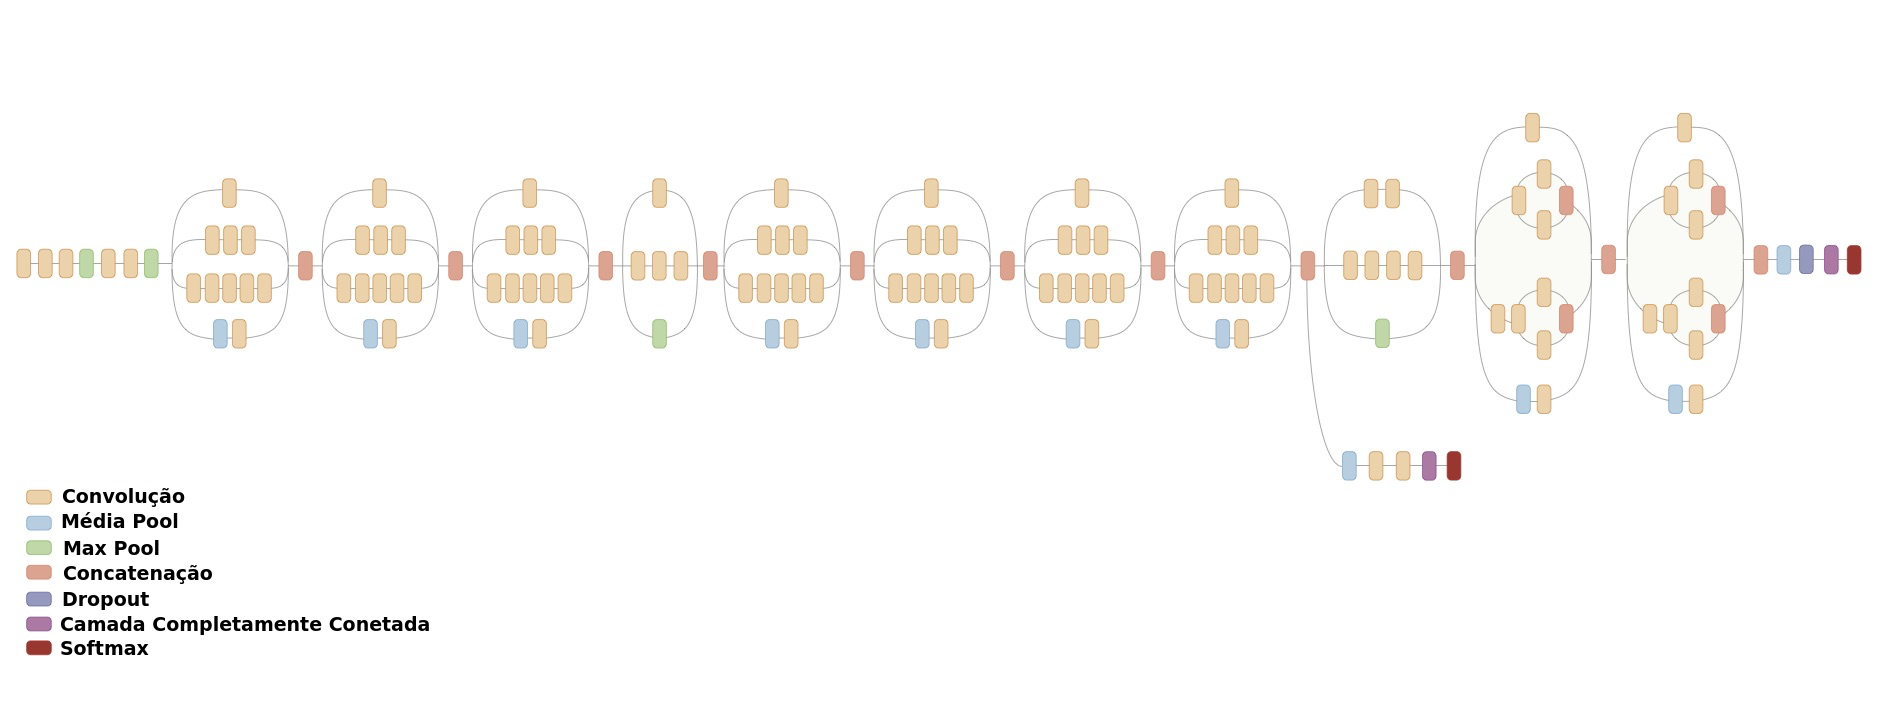
\includegraphics[scale=0.33]{figuras/inceptionV3.png}
\caption{Arquitetura Inception-V3}
\label{fig:inceptionV3}
\end{figure}

\begin{figure}
\centering
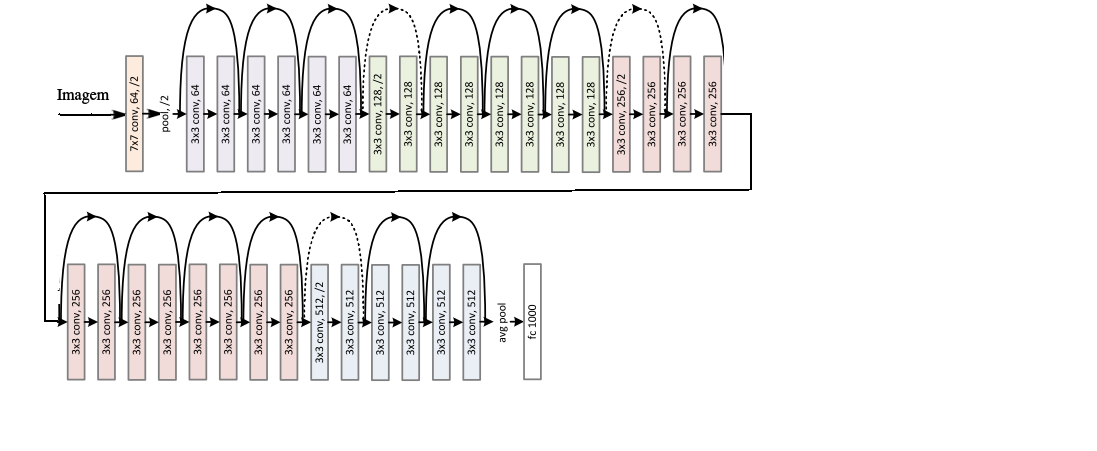
\includegraphics[scale=0.83]{figuras/resnet-34.png}
\caption{Arquitetura ResNet-34}
\label{fig:resnet-34}
\end{figure}



\subsection{Treinamento}
O treinamento consistiu no uso dos materiais descritos na Seção \ref{sec:material} e das bases de treino e teste descritas nas Tabelas \ref{table:basesdivisao} e \ref{table:distclasse}. A estratégia adotada durante a fase de treinamento foi salvar vários modelos enquanto a função de perda convergia para serem utilizadas em comparações. Para todos os experimentos o tamanho de batch foi de 64 imagens e a taxa de aprendizado foi de 0.001 para Alexnet e Inception-V3, no entanto para ResNet-34 foi de 0.1, obviamente isso resultou que a ResNet-34 treinasse mais rápida que as demais, fato que pode ser constatado pela Figura \ref{fig:loss-val}. Esses são os parâmetros padrões de cada arquitetura, por isso não houve qualquer alteração. 

%Para cada arquitetura há uma linha na vertical demarcando o passo em que foi gerado o modelo que obteve as melhores taxas de acurácia, precisão e revocação, e são esses os modelos selecionados para a discussão acerca deste capítulo. Por exemplo, o melhor modelo da arquitetura Alexnet foi gerado no passo 17800, a Residual Net no passo 11250 e a Inception-V3 em 34000. A Figura \ref{fig:acc-val} mostra o gráfico de acurácia na base de teste durante o treinamento. A Figura \ref{fig:loss-val} apresenta o gráfico da função de perda na base de teste ao longo das épocas.


%\begin{figure}
%\centering
%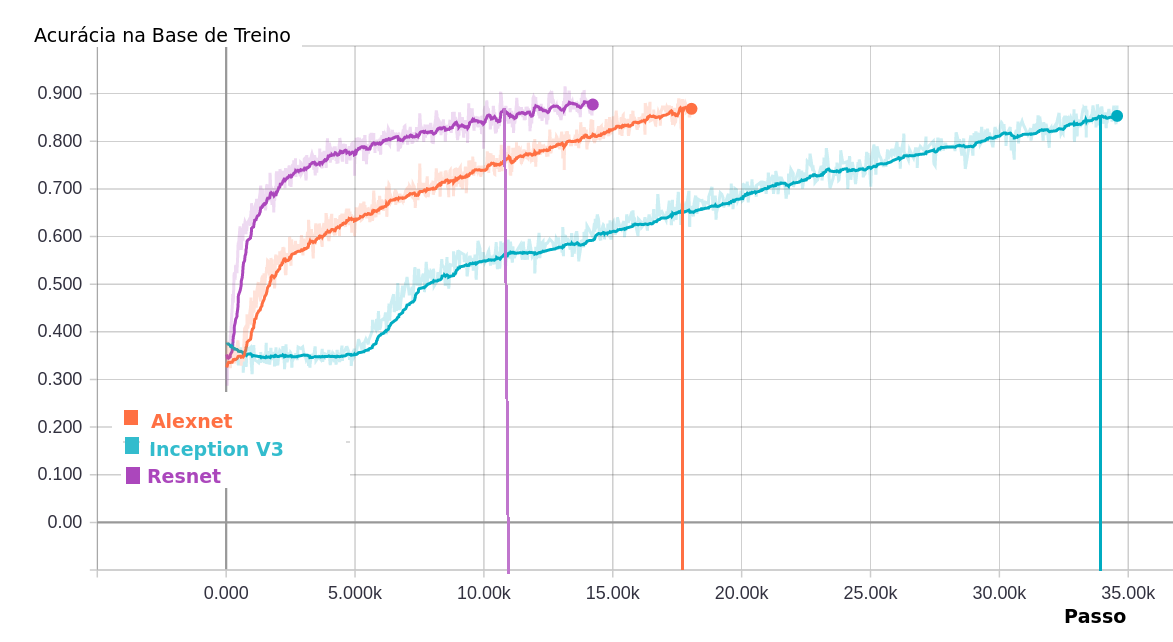
\includegraphics[scale=0.5]{figuras/accuracy.png}
%\caption{Gráfico de Acurácia na Base de Treino. As linhas vertificais indicam o melhor modelo. }
%\label{fig:acc-train}
%\end{figure}

\begin{figure}
\centering
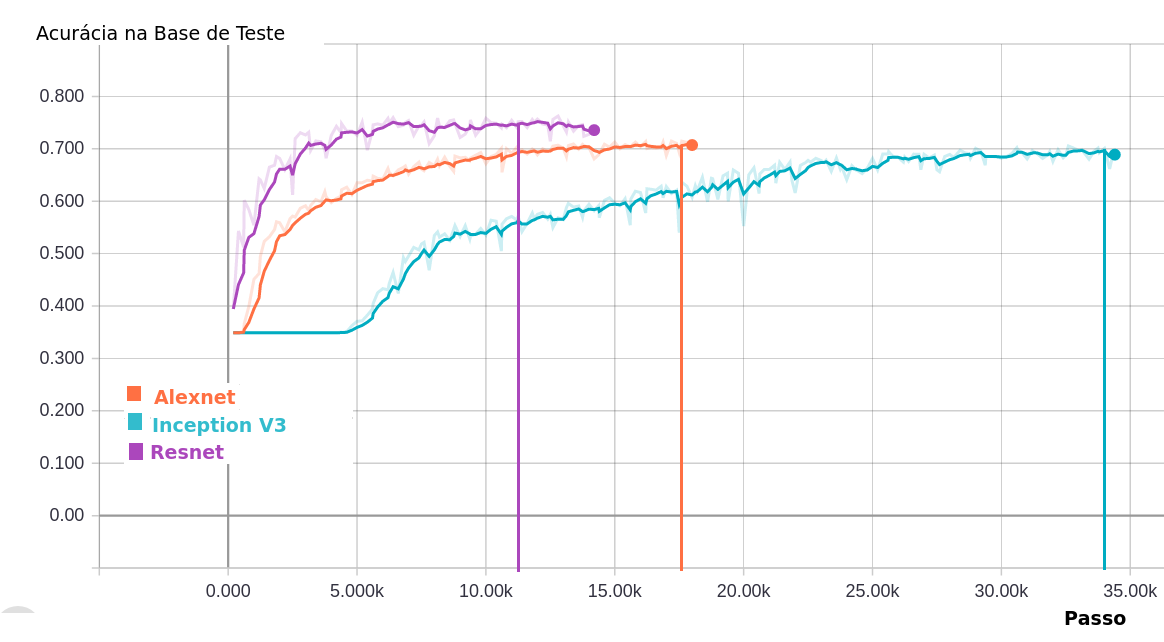
\includegraphics[scale=0.5]{figuras/accuracy_val.png}
\caption{Gráfico de Acurácia na Base de Teste. As linhas vertificais indicam o melhor modelo.}
\label{fig:acc-val}
\end{figure}

%\begin{figure}
%\centering
%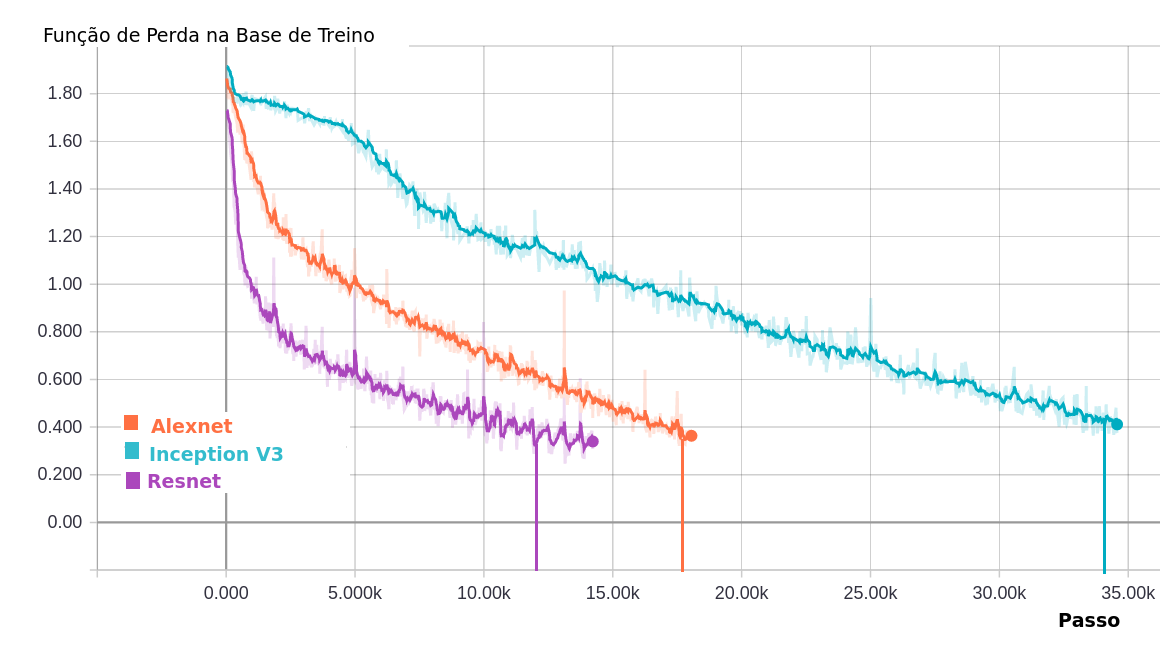
\includegraphics[scale=0.5]{figuras/loss.png}
%\caption{Gráfico da Função de Perda na Base de Treino. As linhas vertificais indicam o melhor modelo.}
%\label{fig:loss-train}
%\end{figure}

\begin{figure}
\centering
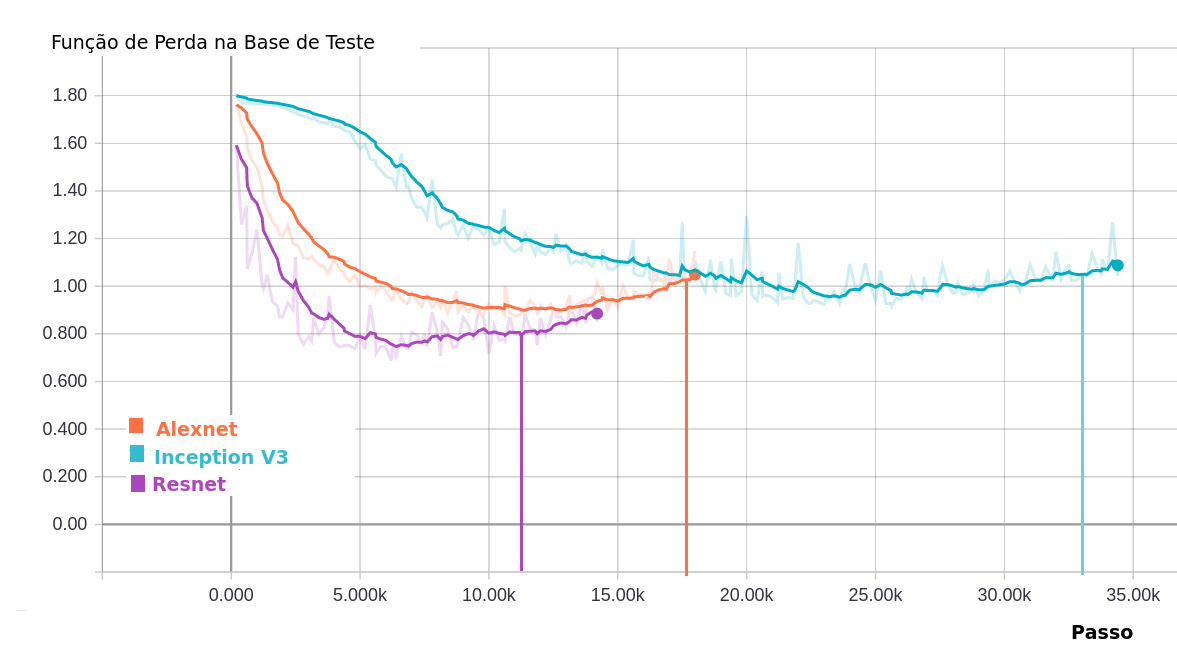
\includegraphics[scale=0.5]{figuras/loss-val.png}
\caption{Gráfico da Função de Perda na Base de Teste. As linhas vertificais indicam o melhor modelo.}
\label{fig:loss-val}
\end{figure}


\subsection{Discussões}




% Please add the following required packages to your document preamble:
% \usepackage{multirow}
\begin{table}[]
\centering
\caption{Resultados experimentais das redes neurais de convolução avaliando a base de validação geral.}
\label{table:resultsexp}
\begin{tabular}{llcccc}
\hline
\textbf{Arquitetura}                & \textbf{Emoção}       & \textbf{Precisão} & \textbf{Revocação} & \textbf{F1-score} & \textbf{Acurácia}               \\ \hline
\multirow{8}{*}{Alexnet}            & Raiva                 & 0.51              & 0.60               & 0.55              & \multirow{8}{*}{0.712}          \\
                                    & Desgosto              & 0.62              & 0.64               & 0.63              &                                 \\
                                    & Medo                  & 0.47              & 0.41               & 0.44              &                                 \\
                                    & Felicidade            & 0.84              & 0.89               & 0.86              &                                 \\
                                    & Tristeza              & 0.64              & 0.50               & 0.56              &                                 \\
                                    & Surpresa              & 0.84              & 0.77               & 0.80              &                                 \\
                                    & Neutralidade          & 0.62              & 0.64               & 0.63              &                                 \\
                                    & Média/Total           & 0.71              & 0.71               & 0.71              &                                 \\ \hline
\multirow{8}{*}{Inception-V3}       & Raiva                 & 0.54              & 0.51               & 0.52              & \multirow{8}{*}{0.701}          \\
                                    & Desgosto              & 0.56              & 0.57               & 0.56              &                                 \\
                                    & Medo                  & 0.47              & 0.42               & 0.44              &                                 \\
                                    & Felicidade            & 0.88              & 0.88               & 0.88              &                                 \\
                                    & Tristeza              & 0.47              & 0.53               & 0.50              &                                 \\
                                    & Surpresa              & 0.85              & 0.79               & 0.82              &                                 \\
                                    & Neutralidade          & 0.59              & 0.62               & 0.61              &                                 \\
                                    & Média/Total           & 0.70              & 0.70               & 0.70              &                                 \\ \hline
\multirow{8}{*}{\textbf{ResNet-34}} & \textbf{Raiva}        & \textbf{0.69}     & \textbf{0.57}      & \textbf{0.62}     & \multirow{8}{*}{\textbf{0.757}} \\
                                    & \textbf{Desgosto}     & \textbf{0.79}     & \textbf{0.66}      & \textbf{0.72}     &                                 \\
                                    & \textbf{Medo}         & \textbf{0.45}     & \textbf{0.50}      & \textbf{0.47}     &                                 \\
                                    & \textbf{Felicidade}   & \textbf{0.90}     & \textbf{0.89}      & \textbf{0.90}     &                                 \\
                                    & \textbf{Tristeza}     & \textbf{0.60}     & \textbf{0.65}      & \textbf{0.63}     &                                 \\
                                    & \textbf{Surpresa}     & \textbf{0.82}     & \textbf{0.86}      & \textbf{0.84}     &                                 \\
                                    & \textbf{Neutralidade} & \textbf{0.67}     & \textbf{0.68}      & \textbf{0.68}     &                                 \\
                                    & \textbf{Média/Total}  & \textbf{0.76}     & \textbf{0.76}      & \textbf{0.76}     &                                 \\ \hline
\end{tabular}
\end{table}




%%%%%%%%%%%%%%%%%%%%%%%%%%%%%%%%%%%%%%%%%%%%%%%%%%%%%%%
%%%%%%%%%%%%%%%%%%%%%%%%%%%%%%%%%%%%%%%%%%%%%%%%%%%%%%%
%%%%%%%%%%%%%%%%%%%%%%%%%%%%%%%%%%%%%%%%%%%%%%%%%%%%%%%
%%%%%%%%%%%%%%%%%%%%%%%%%%%%%%%%%%%%%%%%%%%%%%%%%%%%%%%
%%%%%%%%%%%%%%%%%%%%%%%%%%%%%%%%%%%%%%%%%%%%%%%%%%%%%%%
%%%%%%%%%%%%%%%%%%%%%%%%%%%%%%%%%%%%%%%%%%%%%%%%%%%%%%%



% Please add the following required packages to your document preamble:
% \usepackage{multirow}
\begin{table}[]
\centering
\caption{Resultados experimentais das redes neurais de convolução avaliando a base de validação CK}
\label{table:ck}
\begin{tabular}{llcccc}
\hline
\textbf{Arquitetura}                   & \textbf{Emoção}       & \multicolumn{1}{l}{\textbf{Precisão}} & \multicolumn{1}{l}{\textbf{Revocação}} & \multicolumn{1}{l}{\textbf{F1-score}} & \multicolumn{1}{l}{\textbf{Acurácia}} \\ \hline
\multirow{8}{*}{Alexnet}         & Raiva                 & 0.91                                  & 1                                      & 0.95                                  & \multirow{8}{*}{0.96}                 \\
                                       & Desgosto              & 0.98                                  & 0.97                                   & 0.98                                  &                                       \\
                                       & Medo                  & 0.89                                  & 0.96                                   & 0.92                                  &                                       \\
                                       & Felicidade            & 0.99                                  & 0.99                                   & 0.99                                  &                                       \\
                                       & Tristeza              & 0.98                                  & 0.84                                   & 0.91                                  &                                       \\
                                       & Surpresa              & 1                                     & 0.94                                   & 0.97                                  &                                       \\
                                       & Neutralidade          & 0                                     & 0                                      & 0                                     &                                       \\
                                       & Média/Total           & 0.97                                  & 0.96                                   & 0.96                                  &                                       \\ \hline
\multirow{8}{*}{Inception-V3}     & Raiva                 & 0.93                                  & 0.94                                   & 0.93                                  & \multirow{8}{*}{0.954}                \\
                                       & Desgosto              & 0.96                                  & 0.94                                   & 0.95                                  &                                       \\
                                       & Medo                  & 0.89                                  & 0.96                                   & 0.92                                  &                                       \\
                                       & Felicidade            & 0.99                                  & 0.98                                   & 0.99                                  &                                       \\
                                       & Tristeza              & 0.91                                  & 0.97                                   & 0.94                                  &                                       \\
                                       & Surpresa              & 1                                     & 0.94                                   & 0.97                                  &                                       \\
                                       & Neutralidade          & 0                                     & 0                                      & 0                                     &                                       \\
                                       & Média/Total           & 0.96                                  & 0.95                                   & 0.96                                  &                                       \\ \hline
\multirow{8}{*}{\textbf{ResNet-34}} & \textbf{Raiva}        & \textbf{0.97}                         & \textbf{0.96}                          & \textbf{0.97}                         & \multirow{8}{*}{\textbf{0.969}}       \\
                                       & \textbf{Desgosto}     & \textbf{1}                            & \textbf{0.92}                          & \textbf{0.96}                         &                                       \\
                                       & \textbf{Medo}         & \textbf{0.91}                         & \textbf{0.99}                          & \textbf{0.95}                         &                                       \\
                                       & \textbf{Felicidade}   & \textbf{0.98}                         & \textbf{0.99}                          & \textbf{0.99}                         &                                       \\
                                       & \textbf{Tristeza}     & \textbf{0.94}                         & \textbf{0.96}                          & \textbf{0.95}                         &                                       \\
                                       & \textbf{Surpresa}     & \textbf{0.98}                         & \textbf{0.99}                          & \textbf{0.99}                         &                                       \\
                                       & \textbf{Neutralidade} & \textbf{0}                            & \textbf{0}                             & \textbf{0}                            &                                       \\
                                       & \textbf{Média/Total}  & \textbf{0.97}                         & \textbf{0.97}                          & \textbf{0.97}                         &                                       \\ \hline
\end{tabular}
\end{table}


% Please add the following required packages to your document preamble:
% \usepackage{multirow}
\begin{table}[]
\centering
\caption{Resultados experimentais das redes neurais de convolução avaliando a base de validação FER}
\label{table:fer}
\begin{tabular}{llcccc}
\hline
\textbf{Arquitetura}                   & \textbf{Emoção}       & \multicolumn{1}{l}{\textbf{Precisão}} & \multicolumn{1}{l}{\textbf{Revocação}} & \multicolumn{1}{l}{\textbf{F1-score}} & \multicolumn{1}{l}{\textbf{Acurácia}} \\ \hline
\multirow{8}{*}{Alexnet}         & Raiva                 & 0.39                                  & 0.5                                    & 0.44                                  & \multirow{8}{*}{0.543}                \\
                                       & Desgosto              & 0.45                                  & 0.17                                   & 0.25                                  &                                       \\
                                       & Medo                  & 0.37                                  & 0.33                                   & 0.35                                  &                                       \\
                                       & Felicidade            & 0.74                                  & 0.79                                   & 0.76                                  &                                       \\
                                       & Tristeza              & 0.4                                   & 0.29                                   & 0.34                                  &                                       \\
                                       & Surpresa              & 0.72                                  & 0.64                                   & 0.67                                  &                                       \\
                                       & Neutralidade          & 0.49                                  & 0.52                                   & 0.51                                  &                                       \\
                                       & Média/Total           & 0.54                                  & 0.54                                   & 0.54                                  &                                       \\ \hline
\multirow{8}{*}{Inception-V3}     & Raiva                 & 0.43                                  & 0.4                                    & 0.41                                  & \multirow{8}{*}{0.529}                \\
                                       & Desgosto              & 0.13                                  & 0.25                                   & 0.17                                  &                                       \\
                                       & Medo                  & 0.39                                  & 0.36                                   & 0.37                                  &                                       \\
                                       & Felicidade            & 0.81                                  & 0.77                                   & 0.79                                  &                                       \\
                                       & Tristeza              & 0.29                                  & 0.38                                   & 0.32                                  &                                       \\
                                       & Surpresa              & 0.72                                  & 0.64                                   & 0.68                                  &                                       \\
                                       & Neutralidade          & 0.49                                  & 0.46                                   & 0.47                                  &                                       \\
                                       & Média/Total           & 0.55                                  & 0.53                                   & 0.54                                  &                                       \\ \hline
\multirow{8}{*}{\textbf{ResNet-34}} & \textbf{Raiva}        & \textbf{0.61}                         & \textbf{0.42}                          & \textbf{0.5}                          & \multirow{8}{*}{\textbf{0.604}}       \\
                                       & \textbf{Desgosto}     & \textbf{0.69}                         & \textbf{0.28}                          & \textbf{0.39}                         &                                       \\
                                       & \textbf{Medo}         & \textbf{0.35}                         & \textbf{0.47}                          & \textbf{0.4}                          &                                       \\
                                       & \textbf{Felicidade}   & \textbf{0.87}                         & \textbf{0.81}                          & \textbf{0.84}                         &                                       \\
                                       & \textbf{Tristeza}     & \textbf{0.41}                         & \textbf{0.42}                          & \textbf{0.41}                         &                                       \\
                                       & \textbf{Surpresa}     & \textbf{0.71}                         & \textbf{0.76}                          & \textbf{0.73}                         &                                       \\
                                       & \textbf{Neutralidade} & \textbf{0.56}                         & \textbf{0.61}                          & \textbf{0.58}                         &                                       \\
                                       & \textbf{Média/Total}  & \textbf{0.62}                         & \textbf{0.6}                           & \textbf{0.61}                         &                                       \\ \hline
\end{tabular}
\end{table}



%%%%%%%%%%%%%%%%%%%%%%%%%%%%%%
%%%%%%%%%%%%%%%%%%%%%%
%%%%%%%%%%%%%%%%%%%%%
\begin{comment}
\begin{tiny}
\begin{center}
\begin{longtable}{l|l|l|c|c|c|c}
\caption{Resultados experimentais das redes neurais de convolução avaliando a base de validação individual por cada conjunto de dados.}
\label{table:resultsexpbybase}\\


\hline
\textbf{Base de Dados}         & \textbf{Arquitetura}                   & \textbf{Emoção}       & \multicolumn{1}{l|}{\textbf{Precisão}} & \multicolumn{1}{l|}{\textbf{Revocação}} & \multicolumn{1}{l|}{\textbf{F1-score}} & \multicolumn{1}{l}{\textbf{Acurácia}} \\ \hline
\multirow{24}{*}{CIFE-TEST}    & \multirow{8}{*}{Alexnet}         & Raiva                 & 0.58                                   & 0.70                                    & 0.63                                   & \multirow{8}{*}{0.626}                \\
                               &                                        & Desgosto              & 0.35                                   & 0.38                                    & 0.36                                   &                                       \\
                               &                                        & Medo                  & 0.46                                   & 0.35                                    & 0.40                                   &                                       \\
                               &                                        & Felicidade            & 0.72                                   & 0.80                                    & 0.76                                   &                                       \\
                               &                                        & Tristeza              & 0.72                                   & 0.61                                    & 0.66                                   &                                       \\
                               &                                        & Surpresa              & 0.73                                   & 0.62                                    & 0.67                                   &                                       \\
                               &                                        & Neutralidade          & 0.50                                   & 0.51                                    & 0.50                                   &                                       \\
                               &                                        & Média/Total           & 0.63                                   & 0.63                                    & 0.62                                   &                                       \\ \cline{2-7} 
                               & \multirow{8}{*}{Inception-V3}     & Raiva                 & 0.62                                   & 0.62                                    & 0.62                                   & \multirow{8}{*}{0.613}                \\
                               &                                        & Desgosto              & 0.26                                   & 0.30                                    & 0.28                                   &                                       \\
                               &                                        & Medo                  & 0.47                                   & 0.46                                    & 0.46                                   &                                       \\
                               &                                        & Felicidade            & 0.86                                   & 0.79                                    & 0.83                                   &                                       \\
                               &                                        & Tristeza              & 0.56                                   & 0.54                                    & 0.55                                   &                                       \\
                               &                                        & Surpresa              & 0.70                                   & 0.61                                    & 0.65                                   &                                       \\
                               &                                        & Neutralidade          & 0.45                                   & 0.57                                    & 0.50                                   &                                       \\
                               &                                        & Média/Total           & 0.63                                   & 0.61                                    & 0.62                                   &                                       \\ \cline{2-7} 
                               & \multirow{8}{*}{\textbf{ResNet-34}} & \textbf{Raiva}        & \textbf{0.78}                          & \textbf{0.60}                           & \textbf{0.68}                          & \multirow{8}{*}{\textbf{0.687}}       \\
                               &                                        & \textbf{Desgosto}     & \textbf{0.65}                          & \textbf{0.34}                           & \textbf{0.45}                          &                                       \\
                               &                                        & \textbf{Medo}         & \textbf{0.40}                          & \textbf{0.42}                           & \textbf{0.41}                          &                                       \\
                               &                                        & \textbf{Felicidade}   & \textbf{0.84}                          & \textbf{0.87}                           & \textbf{0.85}                          &                                       \\
                               &                                        & \textbf{Tristeza}     & \textbf{0.66}                          & \textbf{0.71}                           & \textbf{0.69}                          &                                       \\
                               &                                        & \textbf{Surpresa}     & \textbf{0.62}                          & \textbf{0.81}                           & \textbf{0.70}                          &                                       \\
                               &                                        & \textbf{Neutralidade} & \textbf{0.61}                          & \textbf{0.60}                           & \textbf{0.60}                          &                                       \\
                               &                                        & \textbf{Média/Total}  & \textbf{0.69}                          & \textbf{0.69}                           & \textbf{0.68}                          &                                       \\ \hline
\multirow{24}{*}{CIFE-TRAIN}   & \multirow{8}{*}{Alexnet}         & Raiva                 & 0.55                                   & 0.60                                    & 0.58                                   & \multirow{8}{*}{0.624}                \\
                               &                                        & Desgosto              & 0.30                                   & 0.31                                    & 0.30                                   &                                       \\
                               &                                        & Medo                  & 0.50                                   & 0.49                                    & 0.50                                   &                                       \\
                               &                                        & Felicidade            & 0.73                                   & 0.85                                    & 0.79                                   &                                       \\
                               &                                        & Tristeza              & 0.68                                   & 0.60                                    & 0.64                                   &                                       \\
                               &                                        & Surpresa              & 0.71                                   & 0.53                                    & 0.61                                   &                                       \\
                               &                                        & Neutralidade          & 0.54                                   & 0.53                                    & 0.53                                   &                                       \\
                               &                                        & Média/Total           & 0.62                                   & 0.62                                    & 0.62                                   &                                       \\ \cline{2-7} 
                               & \multirow{8}{*}{Inception-V3}     & Raiva                 & 0.58                                   & 0.50                                    & 0.53                                   & \multirow{8}{*}{0.572}                \\
                               &                                        & Desgosto              & 0.21                                   & 0.26                                    & 0.23                                   &                                       \\
                               &                                        & Medo                  & 0.40                                   & 0.47                                    & 0.43                                   &                                       \\
                               &                                        & Felicidade            & 0.83                                   & 0.79                                    & 0.81                                   &                                       \\
                               &                                        & Tristeza              & 0.49                                   & 0.49                                    & 0.49                                   &                                       \\
                               &                                        & Surpresa              & 0.69                                   & 0.54                                    & 0.61                                   &                                       \\
                               &                                        & Neutralidade          & 0.44                                   & 0.53                                    & 0.48                                   &                                       \\
                               &                                        & Média/Total           & 0.59                                   & 0.57                                    & 0.58                                   &                                       \\ \cline{2-7} 
                               & \multirow{8}{*}{\textbf{ResNet-34}} & \textbf{Raiva}        & \textbf{0.71}                          & \textbf{0.61}                           & \textbf{0.66}                          & \multirow{8}{*}{\textbf{0.673}}       \\
                               &                                        & \textbf{Desgosto}     & \textbf{0.44}                          & \textbf{0.22}                           & \textbf{0.30}                          &                                       \\
                               &                                        & \textbf{Medo}         & \textbf{0.46}                          & \textbf{0.52}                           & \textbf{0.49}                          &                                       \\
                               &                                        & \textbf{Felicidade}   & \textbf{0.82}                          & \textbf{0.83}                           & \textbf{0.83}                          &                                       \\
                               &                                        & \textbf{Tristeza}     & \textbf{0.67}                          & \textbf{0.74}                           & \textbf{0.70}                          &                                       \\
                               &                                        & \textbf{Surpresa}     & \textbf{0.60}                          & \textbf{0.75}                           & \textbf{0.67}                          &                                       \\
                               &                                        & \textbf{Neutralidade} & \textbf{0.61}                          & \textbf{0.56}                           & \textbf{0.58}                          &                                       \\
                               &                                        & \textbf{Média/Total}  & \textbf{0.67}                          & \textbf{0.67}                           & \textbf{0.67}                          &                                       \\ \hline
\multirow{24}{*}{CK}           & \multirow{8}{*}{Alexnet}         & Raiva                 & 0.91                                   & 1.00                                    & 0.95                                   & \multirow{8}{*}{0.96}                 \\
                               &                                        & Desgosto              & 0.98                                   & 0.97                                    & 0.98                                   &                                       \\
                               &                                        & Medo                  & 0.89                                   & 0.96                                    & 0.92                                   &                                       \\
                               &                                        & Felicidade            & 0.99                                   & 0.99                                    & 0.99                                   &                                       \\
                               &                                        & Tristeza              & 0.98                                   & 0.84                                    & 0.91                                   &                                       \\
                               &                                        & Surpresa              & 1.00                                   & 0.94                                    & 0.97                                   &                                       \\
                               &                                        & Neutralidade          & 0.00                                   & 0.00                                    & 0.00                                   &                                       \\
                               &                                        & Média/Total           & 0.97                                   & 0.96                                    & 0.96                                   &                                       \\ \cline{2-7} 
                               & \multirow{8}{*}{Inception-V3}     & Raiva                 & 0.93                                   & 0.94                                    & 0.93                                   & \multirow{8}{*}{0.954}                \\
                               &                                        & Desgosto              & 0.96                                   & 0.94                                    & 0.95                                   &                                       \\
                               &                                        & Medo                  & 0.89                                   & 0.96                                    & 0.92                                   &                                       \\
                               &                                        & Felicidade            & 0.99                                   & 0.98                                    & 0.99                                   &                                       \\
                               &                                        & Tristeza              & 0.91                                   & 0.97                                    & 0.94                                   &                                       \\
                               &                                        & Surpresa              & 1.00                                   & 0.94                                    & 0.97                                   &                                       \\
                               &                                        & Neutralidade          & 0.00                                   & 0.00                                    & 0.00                                   &                                       \\
                               &                                        & Média/Total           & 0.96                                   & 0.95                                    & 0.96                                   &                                       \\ \cline{2-7} 
                               & \multirow{8}{*}{\textbf{ResNet-34}} & \textbf{Raiva}        & \textbf{0.97}                          & \textbf{0.96}                           & \textbf{0.97}                          & \multirow{8}{*}{\textbf{0.969}}       \\
                               &                                        & \textbf{Desgosto}     & \textbf{1.00}                          & \textbf{0.92}                           & \textbf{0.96}                          &                                       \\
                               &                                        & \textbf{Medo}         & \textbf{0.91}                          & \textbf{0.99}                           & \textbf{0.95}                          &                                       \\
                               &                                        & \textbf{Felicidade}   & \textbf{0.98}                          & \textbf{0.99}                           & \textbf{0.99}                          &                                       \\
                               &                                        & \textbf{Tristeza}     & \textbf{0.94}                          & \textbf{0.96}                           & \textbf{0.95}                          &                                       \\
                               &                                        & \textbf{Surpresa}     & \textbf{0.98}                          & \textbf{0.99}                           & \textbf{0.99}                          &                                       \\
                               &                                        & \textbf{Neutralidade} & \textbf{0.00}                          & \textbf{0.00}                           & \textbf{0.00}                          &                                       \\
                               &                                        & \textbf{Média/Total}  & \textbf{0.97}                          & \textbf{0.97}                           & \textbf{0.97}                          &                                       \\ \hline
\multirow{24}{*}{FER}          & \multirow{8}{*}{Alexnet}         & Raiva                 & 0.39                                   & 0.50                                    & 0.44                                   & \multirow{8}{*}{0.543}                \\
                               &                                        & Desgosto              & 0.45                                   & 0.17                                    & 0.25                                   &                                       \\
                               &                                        & Medo                  & 0.37                                   & 0.33                                    & 0.35                                   &                                       \\
                               &                                        & Felicidade            & 0.74                                   & 0.79                                    & 0.76                                   &                                       \\
                               &                                        & Tristeza              & 0.40                                   & 0.29                                    & 0.34                                   &                                       \\
                               &                                        & Surpresa              & 0.72                                   & 0.64                                    & 0.67                                   &                                       \\
                               &                                        & Neutralidade          & 0.49                                   & 0.52                                    & 0.51                                   &                                       \\
                               &                                        & Média/Total           & 0.54                                   & 0.54                                    & 0.54                                   &                                       \\ \cline{2-7} 
                               & \multirow{8}{*}{Inception-V3}     & Raiva                 & 0.43                                   & 0.40                                    & 0.41                                   & \multirow{8}{*}{0.529}                \\
                               &                                        & Desgosto              & 0.13                                   & 0.25                                    & 0.17                                   &                                       \\
                               &                                        & Medo                  & 0.39                                   & 0.36                                    & 0.37                                   &                                       \\
                               &                                        & Felicidade            & 0.81                                   & 0.77                                    & 0.79                                   &                                       \\
                               &                                        & Tristeza              & 0.29                                   & 0.38                                    & 0.32                                   &                                       \\
                               &                                        & Surpresa              & 0.72                                   & 0.64                                    & 0.68                                   &                                       \\
                               &                                        & Neutralidade          & 0.49                                   & 0.46                                    & 0.47                                   &                                       \\
                               &                                        & Média/Total           & 0.55                                   & 0.53                                    & 0.54                                   &                                       \\ \cline{2-7} 
                               & \multirow{8}{*}{\textbf{ResNet-34}} & \textbf{Raiva}        & \textbf{0.61}                          & \textbf{0.42}                           & \textbf{0.50}                          & \multirow{8}{*}{\textbf{0.604}}       \\
                               &                                        & \textbf{Desgosto}     & \textbf{0.69}                          & \textbf{0.28}                           & \textbf{0.39}                          &                                       \\
                               &                                        & \textbf{Medo}         & \textbf{0.35}                          & \textbf{0.47}                           & \textbf{0.40}                          &                                       \\
                               &                                        & \textbf{Felicidade}   & \textbf{0.87}                          & \textbf{0.81}                           & \textbf{0.84}                          &                                       \\
                               &                                        & \textbf{Tristeza}     & \textbf{0.41}                          & \textbf{0.42}                           & \textbf{0.41}                          &                                       \\
                               &                                        & \textbf{Surpresa}     & \textbf{0.71}                          & \textbf{0.76}                           & \textbf{0.73}                          &                                       \\
                               &                                        & \textbf{Neutralidade} & \textbf{0.56}                          & \textbf{0.61}                           & \textbf{0.58}                          &                                       \\
                               &                                        & \textbf{Média/Total}  & \textbf{0.62}                          & \textbf{0.60}                           & \textbf{0.61}                          &                                       \\ \hline
\multirow{24}{*}{JAFFE}        & \multirow{8}{*}{Alexnet}         & Raiva                 & 0.62                                   & 0.62                                    & 0.62                                   & \multirow{8}{*}{0.618}                \\
                               &                                        & Desgosto              & 0.57                                   & 0.36                                    & 0.44                                   &                                       \\
                               &                                        & Medo                  & 0.00                                   & 0.00                                    & 0.00                                   &                                       \\
                               &                                        & Felicidade            & 0.93                                   & 0.93                                    & 0.93                                   &                                       \\
                               &                                        & Tristeza              & 0.50                                   & 0.40                                    & 0.44                                   &                                       \\
                               &                                        & Surpresa              & 0.67                                   & 0.80                                    & 0.73                                   &                                       \\
                               &                                        & Neutralidade          & 0.00                                   & 0.00                                    & 0.00                                   &                                       \\
                               &                                        & Média/Total           & 0.65                                   & 0.62                                    & 0.63                                   &                                       \\ \cline{2-7} 
                               & \multirow{8}{*}{Inception-V3}     & Raiva                 & 0.45                                   & 0.62                                    & 0.53                                   & \multirow{8}{*}{0.636}                \\
                               &                                        & Desgosto              & 0.60                                   & 0.27                                    & 0.37                                   &                                       \\
                               &                                        & Medo                  & 0.50                                   & 0.50                                    & 0.50                                   &                                       \\
                               &                                        & Felicidade            & 0.93                                   & 0.93                                    & 0.93                                   &                                       \\
                               &                                        & Tristeza              & 0.44                                   & 0.40                                    & 0.42                                   &                                       \\
                               &                                        & Surpresa              & 0.82                                   & 0.90                                    & 0.86                                   &                                       \\
                               &                                        & Neutralidade          & 0.00                                   & 0.00                                    & 0.00                                   &                                       \\
                               &                                        & Média/Total           & 0.67                                   & 0.64                                    & 0.64                                   &                                       \\ \cline{2-7} 
                               & \multirow{8}{*}{\textbf{ResNet-34}} & \textbf{Raiva}        & \textbf{0.80}                          & \textbf{0.50}                           & \textbf{0.62}                          & \multirow{8}{*}{\textbf{0.654}}       \\
                               &                                        & \textbf{Desgosto}     & \textbf{0.71}                          & \textbf{0.45}                           & \textbf{0.56}                          &                                       \\
                               &                                        & \textbf{Medo}         & \textbf{1.00}                          & \textbf{0.50}                           & \textbf{0.67}                          &                                       \\
                               &                                        & \textbf{Felicidade}   & \textbf{1.00}                          & \textbf{0.64}                           & \textbf{0.78}                          &                                       \\
                               &                                        & \textbf{Tristeza}     & \textbf{0.58}                          & \textbf{0.70}                           & \textbf{0.64}                          &                                       \\
                               &                                        & \textbf{Surpresa}     & \textbf{0.53}                          & \textbf{1.00}                           & \textbf{0.69}                          &                                       \\
                               &                                        & \textbf{Neutralidade} & \textbf{0.00}                          & \textbf{0.00}                           & \textbf{0.00}                          &                                       \\
                               &                                        & \textbf{Média/Total}  & \textbf{0.75}                          & \textbf{0.65}                           & \textbf{0.67}                          &                                       \\ \hline
\multirow{24}{*}{KDEF}         & \multirow{8}{*}{Alexnet}         & Raiva                 & 0.65                                   & 0.59                                    & 0.62                                   & \multirow{8}{*}{0.624}                \\
                               &                                        & Desgosto              & 0.60                                   & 0.79                                    & 0.68                                   &                                       \\
                               &                                        & Medo                  & 0.48                                   & 0.43                                    & 0.45                                   &                                       \\
                               &                                        & Felicidade            & 0.80                                   & 0.93                                    & 0.86                                   &                                       \\
                               &                                        & Tristeza              & 0.52                                   & 0.40                                    & 0.45                                   &                                       \\
                               &                                        & Surpresa              & 0.81                                   & 0.61                                    & 0.70                                   &                                       \\
                               &                                        & Neutralidade          & 0.52                                   & 0.62                                    & 0.57                                   &                                       \\
                               &                                        & Média/Total           & 0.63                                   & 0.62                                    & 0.62                                   &                                       \\ \cline{2-7} 
                               & \multirow{8}{*}{Inception-V3}     & Raiva                 & 0.51                                   & 0.53                                    & 0.52                                   & \multirow{8}{*}{0.587}                \\
                               &                                        & Desgosto              & 0.62                                   & 0.45                                    & 0.52                                   &                                       \\
                               &                                        & Medo                  & 0.54                                   & 0.36                                    & 0.43                                   &                                       \\
                               &                                        & Felicidade            & 0.93                                   & 0.87                                    & 0.90                                   &                                       \\
                               &                                        & Tristeza              & 0.34                                   & 0.50                                    & 0.41                                   &                                       \\
                               &                                        & Surpresa              & 0.76                                   & 0.80                                    & 0.78                                   &                                       \\
                               &                                        & Neutralidade          & 0.54                                   & 0.60                                    & 0.57                                   &                                       \\
                               &                                        & Média/Total           & 0.61                                   & 0.59                                    & 0.59                                   &                                       \\ \cline{2-7} 
                               & \multirow{8}{*}{\textbf{ResNet-34}} & \textbf{Raiva}        & \textbf{0.70}                          & \textbf{0.70}                           & \textbf{0.70}                          & \multirow{8}{*}{\textbf{0.751}}       \\
                               &                                        & \textbf{Desgosto}     & \textbf{0.65}                          & \textbf{0.88}                           & \textbf{0.75}                          &                                       \\
                               &                                        & \textbf{Medo}         & \textbf{0.73}                          & \textbf{0.44}                           & \textbf{0.55}                          &                                       \\
                               &                                        & \textbf{Felicidade}   & \textbf{0.94}                          & \textbf{0.99}                           & \textbf{0.96}                          &                                       \\
                               &                                        & \textbf{Tristeza}     & \textbf{0.69}                          & \textbf{0.70}                           & \textbf{0.70}                          &                                       \\
                               &                                        & \textbf{Surpresa}     & \textbf{0.73}                          & \textbf{0.90}                           & \textbf{0.80}                          &                                       \\
                               &                                        & \textbf{Neutralidade} & \textbf{0.86}                          & \textbf{0.66}                           & \textbf{0.75}                          &                                       \\
                               &                                        & \textbf{Média/Total}  & \textbf{0.76}                          & \textbf{0.75}                           & \textbf{0.74}                          &                                       \\ \hline
\multirow{24}{*}{NOVAEMOTIONS} & \multirow{8}{*}{Alexnet}         & Raiva                 & 0.68                                   & 0.33                                    & 0.44                                   & \multirow{8}{*}{0.857}                \\
                               &                                        & Desgosto              & 0.69                                   & 0.63                                    & 0.66                                   &                                       \\
                               &                                        & Medo                  & 0.57                                   & 0.25                                    & 0.34                                   &                                       \\
                               &                                        & Felicidade            & 0.89                                   & 0.94                                    & 0.92                                   &                                       \\
                               &                                        & Tristeza              & 0.86                                   & 0.73                                    & 0.79                                   &                                       \\
                               &                                        & Surpresa              & 0.90                                   & 0.87                                    & 0.89                                   &                                       \\
                               &                                        & Neutralidade          & 0.76                                   & 0.77                                    & 0.76                                   &                                       \\
                               &                                        & Média/Total           & 0.85                                   & 0.86                                    & 0.85                                   &                                       \\ \cline{2-7} 
                               & \multirow{8}{*}{Inception-V3}     & Raiva                 & 0.30                                   & 0.22                                    & 0.25                                   & \multirow{8}{*}{0.853}                \\
                               &                                        & Desgosto              & 0.68                                   & 0.60                                    & 0.64                                   &                                       \\
                               &                                        & Medo                  & 0.44                                   & 0.15                                    & 0.23                                   &                                       \\
                               &                                        & Felicidade            & 0.90                                   & 0.94                                    & 0.92                                   &                                       \\
                               &                                        & Tristeza              & 0.89                                   & 0.67                                    & 0.77                                   &                                       \\
                               &                                        & Surpresa              & 0.92                                   & 0.88                                    & 0.90                                   &                                       \\
                               &                                        & Neutralidade          & 0.71                                   & 0.77                                    & 0.74                                   &                                       \\
                               &                                        & Média/Total           & 0.85                                   & 0.85                                    & 0.85                                   &                                       \\ \cline{2-7} 
                               & \multirow{8}{*}{\textbf{ResNet-34}} & \textbf{Raiva}        & \textbf{0.54}                          & \textbf{0.33}                           & \textbf{0.41}                          & \multirow{8}{*}{\textbf{0.87}}        \\
                               &                                        & \textbf{Desgosto}     & \textbf{0.85}                          & \textbf{0.65}                           & \textbf{0.74}                          &                                       \\
                               &                                        & \textbf{Medo}         & \textbf{0.73}                          & \textbf{0.15}                           & \textbf{0.25}                          &                                       \\
                               &                                        & \textbf{Felicidade}   & \textbf{0.93}                          & \textbf{0.93}                           & \textbf{0.93}                          &                                       \\
                               &                                        & \textbf{Tristeza}     & \textbf{0.71}                          & \textbf{0.88}                           & \textbf{0.78}                          &                                       \\
                               &                                        & \textbf{Surpresa}     & \textbf{0.93}                          & \textbf{0.89}                           & \textbf{0.91}                          &                                       \\
                               &                                        & \textbf{Neutralidade} & \textbf{0.75}                          & \textbf{0.79}                           & \textbf{0.77}                          &                                       \\
                               &                                        & \textbf{Média/Total}  & \textbf{0.87}                          & \textbf{0.87}                           & \textbf{0.87}                          &                                       \\ \hline
\multirow{24}{*}{RAFD}         & \multirow{8}{*}{Alexnet}         & Raiva                 & 0.66                                   & 0.77                                    & 0.71                                   & \multirow{8}{*}{0.641}                \\
                               &                                        & Desgosto              & 0.58                                   & 0.75                                    & 0.66                                   &                                       \\
                               &                                        & Medo                  & 0.74                                   & 0.58                                    & 0.65                                   &                                       \\
                               &                                        & Felicidade            & 0.72                                   & 0.81                                    & 0.76                                   &                                       \\
                               &                                        & Tristeza              & 0.67                                   & 0.36                                    & 0.47                                   &                                       \\
                               &                                        & Surpresa              & 0.76                                   & 0.73                                    & 0.74                                   &                                       \\
                               &                                        & Neutralidade          & 0.45                                   & 0.38                                    & 0.41                                   &                                       \\
                               &                                        & Média/Total           & 0.65                                   & 0.64                                    & 0.63                                   &                                       \\ \cline{2-7} 
                               & \multirow{8}{*}{Inception-V3}     & Raiva                 & 0.65                                   & 0.72                                    & 0.68                                   & \multirow{8}{*}{0.674}                \\
                               &                                        & Desgosto              & 0.71                                   & 0.65                                    & 0.68                                   &                                       \\
                               &                                        & Medo                  & 0.82                                   & 0.55                                    & 0.66                                   &                                       \\
                               &                                        & Felicidade            & 0.89                                   & 0.87                                    & 0.88                                   &                                       \\
                               &                                        & Tristeza              & 0.46                                   & 0.68                                    & 0.55                                   &                                       \\
                               &                                        & Surpresa              & 0.82                                   & 0.81                                    & 0.81                                   &                                       \\
                               &                                        & Neutralidade          & 0.49                                   & 0.48                                    & 0.49                                   &                                       \\
                               &                                        & Média/Total           & 0.69                                   & 0.67                                    & 0.68                                   &                                       \\ \cline{2-7} 
                               & \multirow{8}{*}{\textbf{ResNet-34}} & \textbf{Raiva}        & \textbf{0.67}                          & \textbf{0.92}                           & \textbf{0.77}                          & \multirow{8}{*}{\textbf{0.775}}       \\
                               &                                        & \textbf{Desgosto}     & \textbf{0.80}                          & \textbf{0.81}                           & \textbf{0.81}                          &                                       \\
                               &                                        & \textbf{Medo}         & \textbf{0.81}                          & \textbf{0.65}                           & \textbf{0.72}                          &                                       \\
                               &                                        & \textbf{Felicidade}   & \textbf{0.87}                          & \textbf{0.94}                           & \textbf{0.90}                          &                                       \\
                               &                                        & \textbf{Tristeza}     & \textbf{0.74}                          & \textbf{0.70}                           & \textbf{0.72}                          &                                       \\
                               &                                        & \textbf{Surpresa}     & \textbf{0.76}                          & \textbf{0.94}                           & \textbf{0.84}                          &                                       \\
                               &                                        & \textbf{Neutralidade} & \textbf{0.80}                          & \textbf{0.44}                           & \textbf{0.57}                          &                                       \\
                               &                                        & \textbf{Média/Total}  & \textbf{0.78}                          & \textbf{0.78}                           & \textbf{0.77}                          &                                       \\ \hline
\end{longtable}
\end{center}
\end{tiny}
\end{comment}

Durante o treinamento vários modelos foram salvos. Adotamos o melhor modelo gerado por cada arquitetura para esta seção, logo vamos discutir a respeito de três modelos eleitos a partir de uma avaliação na base de validação. Os resultados referentes a todos os modelos podem ser consultados no Anexo \ref{anex:results-anexos}. Analisando o anexo somente por arquitetura podemos concluir que o melhor modelo da Alexnet foi gerado no passo 17800, enquanto que a ResidualNet-34 foi no passo 11250 e por fim a Inception-V3 em 34000.   

As Figuras \ref{fig:acc-val} e \ref{fig:loss-val} são a respeito da acurácia na base de teste e da função de perda durante o treinamento. Ambas possuem linhas verticais demarcando os modelos selecionados para a discussão ao longo da seção. Analisando a primeira figura, a taxa de acurácia na base de teste, percebemos que a ResNet-34 no início do treino tem um crescimento semelhante a uma função exponencial e, a partir da interação 5k estabiliza alcançado 76\%. A Alexnet também tem uma curva bastante crescente no início, entretanto foi inferior a ResNet-34 alcançando 70.5\%, uma diferença considerável. A Inception-V3 teve um comportamento diferente, sendo que no início do treino a função ficou estática, e posteriormente, foi crescendo, no entanto assemelhando-se ao crescimento de uma função linear. A Inception-V3 ficou abaixo da Alexnet, alcançando 70\% de acurácia na base de teste. 

A função de perda definida foi a entropia cruzada. A entropia cruzada é apropriada para problemas de classificação. Analisando a Figura \ref{fig:loss-val} podemos interpretar como quanto menor for o valor melhor está sendo o desempenho do classificador, pois esta função é um indicador do erro propagado na rede e o objetivo do gradiente descendente é minimizar estes valores. Logo, quem obteve o menor valor de função de perda foi a Resnet, e consequentemente, a que alcançou melhor desempenho em acurácia. 

Verificando os pontos da função de perda da Inception-V3, é visto que nas primeiras épocas não há uma queda acentuada como nas outras duas. O que coincide com a demora na inclinação da medida de acurácia, obviamente também relacionada a Inception-V3. De acordo com \cite{geron2017hands}, os melhores modelos são os gerados a partir do momento em que a função de perda na base de teste atinge seu valor mínimo até o momento em que começa a crescer. Considerando esta teoria o momento certo de interromper o treinamento é justamente este, quando a função de perda começa a crescer após encontrar o mínimo, este conceito é conhecido como parada antecipada, pois os modelos gerados adiantes possuem \textit{overfitting} (super vícios) na base de treino.

A Tabela \ref{table:resultsexp} apresenta os resultados das redes neurais de convolução avaliando a base de validação geral. Vale ressaltar que a base de validação geral seria uma medição do desempenho dos modelos em cenário real, pois a base de validação não fez parte do treinamento, isto é, são instâncias desconhecidas. Analisamos que a ResNet-34 gerou o modelo que obteve os melhores resultados em todas as métricas: acurácia, precisão, revocação e f1-score, sendo destacada em negrito. A ResNet-34 alcançou 75.7\% em acurácia, enquanto a Alexnet 71.2\% e Inception-V3 70.1\%. Percebemos uma diferença de 4.5\% entre a ResNet-34 e Alexnet caracterizando uma diferença considerável. 

A emoção que a ResNet-34 teve melhor desempenho para reconhecer foi a felicidade alcançando um f1-score em 90\%. Provavelmente pela característica da felicidade ser atribuída a um sorriso. A segunda emoção com melhor resultado foi a surpresa com f1-score em 84\%. Esta emoção tem como marca a boca aberta, outra característica que a rede aprendeu. Este resultado não surpreende, pois essas emoções são duas das três emoções que mais possuem amostragem (consultar Tabela \ref{table:distclasse}). O número de amostra está associado ao aprendizado, teoricamente o cenário ideal é ter a base balanceada ou a quantidade de amostras proporcionais ao mundo real.

Os piores desempenho foram nas emoções medo e raiva. Coincidentemente duas das três emoções que menos tem amostragem. Este resultado não necessariamente foi devido a menor amostragem dessas classes, pois realmente são expressões faciais complicadas. A expressão facial medo não há um padrão bem definido e envolve vários músculos do rosto. Vale ressaltar que a construção de um sistema que possui requisitos de alta precisão nessas duas emoções seja necessário outras fontes de dados além da expressão facial. 

A neutralidade foi uma das três emoções que mais teve amostragem. Entretanto, alcançou somente 68\% de f1-score, portanto um baixo valor. Este resultado pode ser explicado pelo fato da rede neural ter aprendido que a neutralidade consiste em nenhum movimento muscular da face. Caso haja um leve movimento facial a rede tende a classificar em uma das emoções que não seja neutralidade.

Analisando as emoções felicidade e surpresa percebemos que as três arquiteturas obtiveram resultados relativamente aproximados. Lembrando que são duas das três emoções que mais tem amostragem e possuem padrões menos variável como características próprias para diferenciá-las. Entretanto, as outras emoções, com exceção da emoção medo, a ResNet-34 obteve bastante superioridade no desempenho, no qual teoricamente são emoções mais difíceis de aprender, não apenas por ter menos amostragem, mas também por ter padrões menos definidos e variáveis. A emoção medo foi praticamente empate com resultado ruim em todas as arquiteturas. 


%Estes resultados supõe que a ResNet é uma rede que se adequa ao problema de reconhecimento de emoção via expressão facial.


%As Tabelas \ref{table:cife-test}, \ref{table:cife-train}, \ref{table:ck}, \ref{table:fer}, \ref{table:jaffe}, \ref{table:kdef}, \ref{table:novaemotions} e \ref{table:rafd} apresentam os resultados das redes neurais de conovolução avaliando as bases de validação: \textit{CIFE-Train}, \textit{CIFE-Test}, \textit{CK}, \textit{FER}, \textit{JAFFE}, \textit{KDEF}, \textit{NovaEmotions} e \textit{RAFD}, respectivamente, 

As Tabelas \ref{table:ck} e \ref{table:fer} apresentam os resultados das redes neurais de convolução avaliando as bases de validação: \textit{CK} e \textit{FER}. Essas duas bases foram escolhidas por serem as mais utilizadas na literatura e por uma possuir característica de imagens capturadas no laboratório (CK) e a outra na natureza (FER). No Anexo \ref{anex:results-anexos-val} pode ser consultado os resultados para as demais bases: \textit{CIFE-Train}, \textit{CIFE-Test}, \textit{JAFFE}, \textit{KDEF}, \textit{NovaEmotions} e \textit{RAFD}. 

A base CK teve ótimos resultados nas três arquiteturas (ver Tabela \ref{table:ck}). No entanto, a ResNet-34 foi a melhor chegando a 96.9\% de acurácia. O que acarretou este resultado expressivo nas três arquiteturas foi o fato desta base ser laboratorial. Neste caso, configura um cenário perfeito onde as imagens não tem ruídos, pouca variabilidade, distância próxima e fixa da câmera, iluminação ideal, pouca angulação da face, os atores emitindo as emoções com alta intensidade e rotulação correta da base. 

Nos trabalhos de \cite{art1}, \cite{art11} e \cite{art7} obtiveram  99.1\%, 98.7\% e 97.3\%, respectivamente, contudo vale destacar que estes trabalhos treinaram e testaram somente com a base CK, que tende a ter melhor desempenho de fato, pois se especializaram em reconhecer imagens dessa base e laboratoriais. Outro ponto relevante é que não fica claro se esses resultados são referentes a base de teste ou validação. Nosso trabalho alcançou 96.9\% na base de validação, ou seja, próximo dos resultados acima, com a combinação de várias bases inclusive de características de imagens na natureza. Além disso, nesta base não há amostragem da emoção neutralidade, entretanto em nosso trabalho foi incluída esta emoção. Isto acarretou o aumento da chance de existir uma confusão entre a neutralidade e qualquer outra emoção da base, enquanto os outros trabalhos não apoiaram o reconhecimento para tal. Contudo, não houve qualquer confusão em atribuir como neutralidade qualquer imagem oriunda da base CK, o que está correto, pois nessa base não há neutralidade. Podemos concluir que imagens fotografadas na natureza para treinamento não influenciam negativamente o desempenho do classificador atuando em imagens laboratoriais estilo CK. 

O resultado da base FER não foi tão bom (consultar Tabela \ref{table:fer}). Analisando a acurácia a ResNet-34 alcançou 60.4\%, enquanto a Alexnet 54.3\% e a Inception-V3 52.9\%. Percebemos que em ambos os casos há uma diferença de performance acima de 6\% entre a ResNet-34 com as outras arquiteturas. Isto supõe que a base FER é uma base difícil para ser aprendida e classificada. O que não é surpresa, pois essa base é composta por imagens oriundas da natureza, no qual não há um padrão de iluminação, variação do fundo do ambiente, distância fixa com câmera, faces com fortes movimentações e emoções com grau de intensidades diferentes. É válido ressaltar que o fato desta base possuir emoções com variação na intensidade pode acarretar imagens com baixa emoção, caracterizando que essas instâncias se encontrem em uma região de confusão, onde não é tão evidente distinguir qual é a emoção havendo sobreposição. Por isso, esta base possui algumas imagens com rótulos questionáveis. Tanto é que pesquisadores da Microsoft resolveram usar as plataformas da empresa para re-rotular a base FER gerando uma nova base denominada FER+ \citep{barsoum2016training}.      

Comparando os resultados com a comunidade científica, o trabalho de \cite{art7} alcançou 76.9\%, \cite{kim2016fusing} conseguiu 73.73\% e \cite{art5} atingiu 65\%, todos estes trabalhos utilizaram a base FER para treino e teste. Obviamente por treinarem e testarem somente nesta base os modelos gerados especializaram-se nas características dessa base. Um dos motivos para nosso trabalho ter ficado tão atrás foi que as imagens laboratorias pode influenciar negativamente no ajuste de pesos para classificar imagens na natureza. Outro fator prejudicial foi a ausência de técnicas como normalização do brilho e constrate, alinhamento da face e aumentação de dados. Estas técnicas fazem parte da solução proposta, entretanto ainda precisam ser implementadas. A idéia é tornar a abordagem mais robusta para lidar com cenários de uso reais, e consequentemente, com imagens advindas da natureza.    

Portanto, o estudo comparativo mostrou que a ResNet-34 foi a melhor arquitetura. Verificamos que houve praticamente um empate entre a Alexnet e a Inception-V3, enquanto a ResNet-34 sempre esteve a frente em desempenho com uma diferença considerável. Vale destacar que a base CK, uma base de origem laboratorial, nosso trabalho obteve taxas próximas da comunidade científica. Entretanto, na base FER, uma base oriunda da natureza, ficamos distantes dos resultados da literatura. Porém, é de se considerar que a nossa abordagem ainda não está totalmente implementada. Esperamos que o desenvolvimento dos componentes faltantes tornem a nossa solução mais robusta para casos de usos complexos na natureza. 

\section{Resumo}\label{sec:considera}
Nossos resultados parciais foi iniciado com uma prova de conceito na área de educação. Esta prova de conceito foi fundamental para a evolução desta proposta. Em uso de cenário real percebemos a dificuldade de funcionar tais aplicações. Realizamos uma análise das emoções dos estudantes com seu desempenho em um teste escolar. As emoções foram reconhecidas usando um serviço em nuvem. Percebemos como reconhecer emoções por meio de câmeras, uma coleta não intrusiva, pode colaborar para transformar sistemas inteligentes mais robustos. Contudo, estamos desenvolvendo nosso próprio reconhecedor de emoção. O primeiro passo foi um estudo comparativo entre as arquiteuras Alexnet, Inception-V3 e ResNet. Concluímos que a ResNet obteve os melhores resultados. Em imagens laboratoriais, a ResNet foi muito bem aproximado-se dos baselines. Percebemos que há uma série de desafios em classificar imagens da natureza, no qual a ResNet ainda não obteve os resultados desejados. Porém, a abordagem proposta ainda não está totalmente desenvolvida. Esperamos ter um sistema robusto e preciso para lidar com situações complexas de classificação.      

%Foi possível verificar que o reconhecedor de emoção tem muita aplicação, iniciamos nossa aplicação no cenário real em uma prova de conceito na área de educação, no qual há muitas utilidades. Esta prova de conceito nos deu norte para a evolução desta proposta. Consequentemente foi iniciado o desenvolvimento do reconhecedor que esta proposta pretende gerar como contribuição. Há muitos trabalhos futuros, principalmente combinar as diversas técnicas de pré-processamento com as diversas arquiteturas de RNC juntamente com as bases de dados. A área de aprendizagem de máquina costuma ser bastante experimental e aparentemente temos bastante configuração de experimento para testar, até encontrar a melhor taxa de aprendizado da RNC.